\documentclass{article}%
\usepackage[T1]{fontenc}%
\usepackage[utf8]{inputenc}%
\usepackage{lmodern}%
\usepackage{textcomp}%
\usepackage{lastpage}%
%
\usepackage{amsmath}%
\usepackage{amssymb}%
\usepackage{amsfonts}%
\usepackage{graphicx}%
\usepackage{hyperref}%
\usepackage{tikz}%
\usepackage{pgfplots}%
\usetikzlibrary{math}%
\title{IME 2027 - Química\thanks{This exam was solved and automatically generated with gpt-resolve: \url{https://github.com/lgabs/gpt-resolve}}}%
\author{claude{-}haiku{-}5{-}5 (solver) + claude{-}haiku{-}5{-}5 (judge)}%
\date{November 10, 2026}%
%
\begin{document}%
\normalsize%
\maketitle%
\section*{Questão 1}

\section*{Solução}

\textbf{Dados e hipóteses.} Esta questão usa apenas as massas molares, obtidas da Tabela Periódica da prova. Os demais dados da Folha de Dados ($R$, constantes crioscópicas, densidades, $\ln 2$ e $\ln 5$) não são necessários. Adotam-se as seguintes hipóteses:
\begin{itemize}
\item[(i)] Rendimento de $100\%$ em todas as etapas, isto é, cálculo estequiométrico teórico.
\item[(ii)] O $\mathrm{HCl}$ concentrado está em quantidade suficiente para a reação. Esta é uma premissa: o enunciado não informa a quantidade de $\mathrm{HCl}$, e não ser reagente não implica estar em excesso. Como a pergunta é sobre o $\mathrm{MnO_2}$, ele é o reagente cuja quantidade determina o $\mathrm{Cl_2}$ gerado.
\item[(iii)] O $\mathrm{Cl_2}$ é a quantidade mínima necessária, a que a estequiometria exige para oxidar todo o $\mathrm{Br^{-}}$, como pede o enunciado (``o cloro necessário''). Excesso de cloro fica fora do modelo: na prática, ele poderia converter parte do $\mathrm{Br_2}$ em $\mathrm{BrCl}$ ($\mathrm{Cl_2 + Br_2 \rightleftharpoons 2\,BrCl}$), o que alteraria a relação $2\,\mathrm{NaBr} : 1\,\mathrm{Cl_2}$ usada aqui.
\item[(iv)] Os $2{,}06\ \mathrm{g}$ são de $\mathrm{NaBr}$ puro, de modo que todo o bromo está na forma $\mathrm{Br^{-}}$.
\item[(v)] A massa pedida é a de $\mathrm{MnO_2}$ puro. O teor de $\mathrm{MnO_2}$ na pirolusita não é dado.
\end{itemize}

\textbf{1. Reações envolvidas.}

\textbf{(a) Geração de cloro.} Em meio ácido, o manganês passa do Nox $+4$ (no $\mathrm{MnO_2}$) a $+2$ (no $\mathrm{Mn^{2+}}$), ganhando $2\,\mathrm{e^{-}}$ (redução). Dois íons $\mathrm{Cl^{-}}$ passam a $\mathrm{Cl_2}$ (Nox $0$), perdendo $2\,\mathrm{e^{-}}$ (oxidação). As semirreações são:
\begin{align*}
\mathrm{MnO_2 + 4\,H^{+} + 2\,e^{-}} &\longrightarrow \mathrm{Mn^{2+} + 2\,H_2O} \\
\mathrm{2\,Cl^{-}} &\longrightarrow \mathrm{Cl_2 + 2\,e^{-}}
\end{align*}
Somando as duas e acrescentando $2\,\mathrm{Cl^{-}}$ a cada membro, o $\mathrm{Mn^{2+}}$ passa a ter os dois íons $\mathrm{Cl^{-}}$ que formam o $\mathrm{MnCl_2}$. Como os íons $\mathrm{H^{+}}$ e $\mathrm{Cl^{-}}$ vêm do $\mathrm{HCl}$ ($4\,\mathrm{HCl} \to 4\,\mathrm{H^{+}} + 4\,\mathrm{Cl^{-}}$):
\begin{align*}
\mathrm{MnO_2 + 4\,HCl} &\longrightarrow \mathrm{MnCl_2 + Cl_2 + 2\,H_2O}
\end{align*}
Nem todo o $\mathrm{HCl}$ é oxidado: dois dos quatro $\mathrm{Cl^{-}}$ formam $\mathrm{Cl_2}$, e os outros dois formam $\mathrm{MnCl_2}$. Os quatro $\mathrm{H^{+}}$ formam as duas moléculas de $\mathrm{H_2O}$.

Conferência atômica: $\mathrm{Mn}$: $1 = 1$; $\mathrm{O}$: $2 = 2$; $\mathrm{H}$: $4 = 4$; $\mathrm{Cl}$: $4 = 2 + 2$.

Balancear apenas pelos elétrons não basta: $\mathrm{MnO_2 + 2\,HCl \longrightarrow MnCl_2 + Cl_2 + H_2O}$ também tem $2 = 2$ elétrons, mas não fecha, pois o $\mathrm{Cl}$ tem $2$ à esquerda e $4$ à direita, e o $\mathrm{O}$ tem $2$ à esquerda e $1$ à direita.

\textbf{(b) Liberação do bromo.} O $\mathrm{Cl_2}$ oxida o $\mathrm{Br^{-}}$ a $\mathrm{Br_2}$ (cada $\mathrm{Br_2}$ perde $2\,\mathrm{e^{-}}$), e é reduzido a $2\,\mathrm{Cl^{-}}$ (ganha $2\,\mathrm{e^{-}}$):
\begin{align*}
\mathrm{2\,NaBr + Cl_2} &\longrightarrow \mathrm{2\,NaCl + Br_2}
\end{align*}
Conferência atômica: $\mathrm{Na}$: $2 = 2$; $\mathrm{Br}$: $2 = 2$; $\mathrm{Cl}$: $2 = 2$.

\textbf{(c) Equação global.} Somando (a) e (b), o $\mathrm{Cl_2}$ aparece nos dois membros e se cancela:
\begin{align*}
\mathrm{MnO_2 + 4\,HCl + 2\,NaBr} &\longrightarrow \mathrm{MnCl_2 + 2\,NaCl + Br_2 + 2\,H_2O}
\end{align*}
Conferência atômica: $\mathrm{Mn}$: $1 = 1$; $\mathrm{O}$: $2 = 2$; $\mathrm{H}$: $4 = 4$; $\mathrm{Na}$: $2 = 2$; $\mathrm{Br}$: $2 = 2$; $\mathrm{Cl}$: $4 = 2 + 2$.

\textbf{2. Relação estequiométrica.} Pela equação global, $1\ \mathrm{mol}$ de $\mathrm{MnO_2}$ reage com $2\ \mathrm{mol}$ de $\mathrm{NaBr}$. Pela cadeia (a)+(b), $n(\mathrm{MnO_2}) = n(\mathrm{Cl_2})$ e $n(\mathrm{Cl_2}) = n(\mathrm{NaBr})/2$. Logo,
\[ n(\mathrm{MnO_2}) = \frac{n(\mathrm{NaBr})}{2}. \]

\textbf{3. Massas molares} (Tabela Periódica da prova: $\mathrm{Na} = 22{,}990$; $\mathrm{Br} = 79{,}904$; $\mathrm{Mn} = 54{,}938$; $\mathrm{O} = 15{,}999$):
\[ M(\mathrm{NaBr}) = 22{,}990 + 79{,}904 = 102{,}894\ \mathrm{g\cdot mol^{-1}}, \qquad M(\mathrm{MnO_2}) = 54{,}938 + 2\cdot 15{,}999 = 86{,}936\ \mathrm{g\cdot mol^{-1}}. \]

\textbf{4. Cálculo.} Os valores intermediários são mantidos com mais algarismos, sem arredondamento precoce:
\[ n(\mathrm{NaBr}) = \frac{2{,}06\ \mathrm{g}}{102{,}894\ \mathrm{g\cdot mol^{-1}}} \approx 2{,}002\times 10^{-2}\ \mathrm{mol}, \qquad n(\mathrm{MnO_2}) = \frac{2{,}002\times 10^{-2}\ \mathrm{mol}}{2} \approx 1{,}001\times 10^{-2}\ \mathrm{mol}. \]
\[ m(\mathrm{MnO_2}) = n(\mathrm{MnO_2})\cdot M(\mathrm{MnO_2}) \approx 1{,}001\times 10^{-2}\ \mathrm{mol}\cdot 86{,}936\ \mathrm{g\cdot mol^{-1}} \approx 0{,}870\ \mathrm{g}. \]
Forma direta equivalente: $m(\mathrm{MnO_2}) = \dfrac{2{,}06\cdot 86{,}936}{2\cdot 102{,}894}\ \mathrm{g} \approx 0{,}8703\ \mathrm{g}$.

Algarismos significativos: o dado $2{,}06\ \mathrm{g}$ tem três algarismos significativos, e a massa molar tem precisão maior, então o resultado é $0{,}870\ \mathrm{g}$.

\textbf{5. Conferência.}
\begin{itemize}
\item Unidades: $\mathrm{g}/(\mathrm{g\cdot mol^{-1}}) = \mathrm{mol}$ e $\mathrm{mol}\cdot\mathrm{g\cdot mol^{-1}} = \mathrm{g}$. Correto.
\item Balanço do bromo: o bromo em $2{,}06\ \mathrm{g}$ de $\mathrm{NaBr}$ é $2{,}06\cdot 79{,}904/102{,}894 \approx 1{,}600\ \mathrm{g}$. O $\mathrm{Br_2}$ formado a partir de $1{,}001\times 10^{-2}\ \mathrm{mol}$ de $\mathrm{MnO_2}$ tem massa $1{,}001\times 10^{-2}\cdot 159{,}808 \approx 1{,}600\ \mathrm{g}$. Logo, todo o bromo é liberado.
\item Erros comuns: (1) usar a razão $1:1$ entre $\mathrm{NaBr}$ e $\mathrm{Cl_2}$ levaria a $n(\mathrm{MnO_2}) = 2{,}002\times 10^{-2}\ \mathrm{mol}$ e a $1{,}74\ \mathrm{g}$, o que ignora que $1\ \mathrm{mol}$ de $\mathrm{Cl_2}$ oxida $2\ \mathrm{mol}$ de $\mathrm{Br^{-}}$. (2) Usar $2\,\mathrm{Cl_2}$ por $\mathrm{MnO_2}$ levaria a $0{,}435\ \mathrm{g}$, o que ignora que $1\ \mathrm{mol}$ de $\mathrm{MnO_2}$ gera $1\ \mathrm{mol}$ de $\mathrm{Cl_2}$. (3) Balancear só pelos elétrons não altera a razão $\mathrm{MnO_2 : Cl_2}$, mas gera uma equação química incorreta, como visto em (a).
\item Arredondamento: com $\mathrm{Br} = 80{,}00$ em vez de $79{,}904$, a massa muda menos de $0{,}001\ \mathrm{g}$; o resultado não depende desse arredondamento.
\item Minério: se o teor de $\mathrm{MnO_2}$ na pirolusita fosse $p$ (fração mássica), seriam necessários $0{,}870\ \mathrm{g}/p$ de minério. Como $p$ não é dado, a resposta refere-se ao $\mathrm{MnO_2}$ puro.
\end{itemize}

\textbf{Resposta.} São necessários cerca de $0{,}870\ \mathrm{g}$ de $\mathrm{MnO_2}$ puro ($\approx 1{,}00\times 10^{-2}\ \mathrm{mol}$), na proporção $1\,\mathrm{MnO_2} : 2\,\mathrm{NaBr}$, com $\mathrm{MnO_2} + 4\,\mathrm{HCl} \rightarrow \mathrm{MnCl_2} + \mathrm{Cl_2} + 2\,\mathrm{H_2O}$ e $2\,\mathrm{NaBr} + \mathrm{Cl_2} \rightarrow 2\,\mathrm{NaCl} + \mathrm{Br_2}$.

ANSWER: $m(\mathrm{MnO_2}) \approx 0{,}870\ \mathrm{g}$%
\newpage%
\section*{Questão 2}

\section*{Solução}

\noindent\textbf{Hipóteses e convenções.}
\begin{itemize}
  \item Gás ideal, $n = 1$ mol, com $PV = RT$ em cada estado de equilíbrio.
  \item Para gás ideal, $U = U(T)$ (lei de Joule), com $C_V > 0$, ou seja, $U$ cresce estritamente com $T$.
  \item Etapas I e III: quase-estáticas (lentas), com a pressão do gás igual à externa a cada instante. Logo $W = \int P\,dV$ com $P = RT/V$. Como são isotermas, $\Delta U = 0$.
  \item Etapas II e IV: $Q = 0$ (enunciado) e irreversíveis. Os estados intermediários não são de equilíbrio, então $P$ não tem valor definido nesses trechos e $\int P\,dV$ não se aplica. Usa-se a primeira lei.
  \item Convenção: $W$ é o trabalho realizado pelo gás e $Q$ é o calor recebido, com $Q = \Delta U + W$. Em trechos irreversíveis, $W = \int P_{ext}\,dV$. Numa compressão $W < 0$ e numa expansão $W > 0$.
\end{itemize}

Estados: $1 = (P_1,V_1,T_1)$, $2 = (P_2,V_2,T_2)$, $3 = (P_3,V_3,T_3)$, $4 = (P_4,V_4,T_4)$. As etapas I e III são isotermas, logo $T_2 = T_1$ e $T_4 = T_3$. Também $P_1V_1 = RT_1$ e $P_4V_4 = RT_3$. Pelo sentido de cada etapa: $V_2 < V_1$ (I comprime), $V_3 < V_2$ (II comprime), $V_4 > V_3$ (III expande) e $V_1 > V_4$ (IV expande até o estado 1).

Na etapa II, $W_2 < 0$ (compressão), e a primeira lei com $Q_2 = 0$ dá $\Delta U_2 = -W_2 > 0$. Com $C_V > 0$, isso implica $T_3 > T_1$.

\noindent\textbf{a) Esboço do gráfico $P \times V$.}
\begin{itemize}
  \item \textbf{Etapa I} ($1 \to 2$): isoterma quase-estática a $T_1$, ramo da hipérbole $PV = P_1V_1$ (Boyle). Compressão: $V_2 < V_1$ e $P_2 > P_1$.
  \item \textbf{Etapa II} ($2 \to 3$): compressão rápida, com $Q = 0$ e irreversível. Os estados intermediários não são de equilíbrio, então não existe curva $P \times V$ para o trecho. Ele é representado apenas por um segmento tracejado ligando os extremos 2 e 3. Não se desenha a adiabática reversível $PV^{\gamma} = \text{cte}$, cuja inclinação $-\gamma P/V$ é mais íngreme que a da isoterma, $-P/V$, pois $\gamma > 1$; esse não é o trajeto percorrido. Resultados: $T_3 > T_1$, $V_3 < V_2$ e $P_3 = RT_3/V_3 > RT_1/V_2 = P_2$.
  \item \textbf{Etapa III} ($3 \to 4$): isoterma quase-estática a $T_3$, hipérbole $PV = RT_3$, acima da de $T_1$ porque $T_3 > T_1$. Expansão: $V_4 > V_3$ e $P_4 < P_3$.
  \item \textbf{Etapa IV} ($4 \to 1$): expansão rápida, com $Q = 0$ e irreversível, também representada por segmento tracejado. Como o estado final é 1, $V_1 > V_4$. Além disso, $P_4/P_1 = (T_3/T_1)(V_1/V_4) > 1$, logo $P_1 < P_4$.
\end{itemize}

Assim, $V_3 < V_2 < V_1$ e $V_3 < V_4 < V_1$. $P_1$ é a menor pressão e $P_3$ a maior. Os dados não fixam a ordem entre $V_2$ e $V_4$, nem entre $P_2$ e $P_4$. A figura mostra um caso possível.

\begin{center}
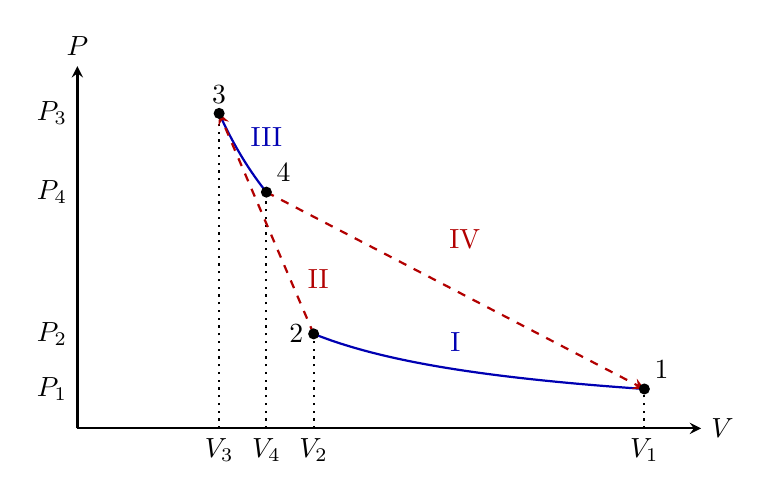
\begin{tikzpicture}[x=0.6cm, y=0.1cm, >=stealth, thick]
  % eixos
  \draw[->] (0,0) -- (13.2,0) node[right] {$V$};
  \draw[->] (0,0) -- (0,46) node[above] {$P$};
  % projecoes dos estados sobre o eixo V
  \draw[dotted] (3,0) -- (3,40);
  \draw[dotted] (4,0) -- (4,30);
  \draw[dotted] (5,0) -- (5,12);
  \draw[dotted] (12,0) -- (12,5);
  \node[below] at (3,0) {$V_3$};
  \node[below] at (4,0) {$V_4$};
  \node[below] at (5,0) {$V_2$};
  \node[below] at (12,0) {$V_1$};
  \node[left] at (0,5) {$P_1$};
  \node[left] at (0,12) {$P_2$};
  \node[left] at (0,30) {$P_4$};
  \node[left] at (0,40) {$P_3$};
  % etapas I e III: isotermas quase-estaticas (curvas P x V)
  \draw[blue!70!black, domain=5:12, samples=60] plot (\x,{60/\x});
  \draw[blue!70!black, domain=3:4, samples=30] plot (\x,{120/\x});
  % etapas II e IV: trajetos irreversiveis com Q=0, sem curva P x V (segmento tracejado entre os extremos)
  \draw[red!70!black, dashed, ->] (5,12) -- (3,40);
  \draw[red!70!black, dashed, ->] (4,30) -- (12,5);
  % estados
  \fill (12,5) circle (2pt) node[above right] {$1$};
  \fill (5,12) circle (2pt) node[left] {$2$};
  \fill (3,40) circle (2pt) node[above] {$3$};
  \fill (4,30) circle (2pt) node[above right] {$4$};
  % rotulos das etapas
  \node[blue!70!black] at (8,11) {I};
  \node[red!70!black] at (5.1,19) {II};
  \node[blue!70!black] at (4,37) {III};
  \node[red!70!black] at (8.2,24) {IV};
\end{tikzpicture}
\end{center}

\noindent Legenda: em azul, as isotermas quase-estáticas (etapas I e III), que são curvas $P \times V$. Em vermelho tracejado, as etapas II e IV: trajetos irreversíveis com $Q = 0$, sem curva $P \times V$ definida. O tracejado não representa trabalho, ou seja, a área sob ele não é $W_2$ nem $W_4$. Os valores são ilustrativos ($nRT_1 = 60$ e $nRT_3 = 120$, em unidades de $P \times V$). O percurso $1 \to 2 \to 3 \to 4 \to 1$ é horário, mas isso não indica motor: com estes valores, $W_1 + W_3 = 60\ln\frac{5}{12} + 120\ln\frac{4}{3} \approx -18$, negativo, porque $V_2V_4 \neq V_1V_3$ (ver verificações).

\noindent\textbf{b) Demonstração de $W_{tot} = W_1 + W_3$.}

\noindent\emph{Etapas I e III (isotermas quase-estáticas).} Com $P = RT/V$ e $\Delta U = 0$, pela primeira lei $Q = W$ nessas etapas:

\begin{align*}
W_1 &= \int_{V_1}^{V_2} \frac{RT_1}{V}\,dV = RT_1\ln\frac{V_2}{V_1} = P_1V_1\ln\frac{V_2}{V_1} \quad (<0),\\
W_3 &= \int_{V_3}^{V_4} \frac{RT_3}{V}\,dV = RT_3\ln\frac{V_4}{V_3} = P_4V_4\ln\frac{V_4}{V_3} \quad (>0).
\end{align*}

\noindent\emph{Etapas II e IV (irreversíveis, $Q = 0$).} A primeira lei dá $W = -\Delta U$ em cada trecho, qualquer que seja o caminho. Não se usa $\int P\,dV$ aqui:

\begin{align*}
W_2 &= -\Delta U_2 = -\bigl[U(T_3) - U(T_1)\bigr], \\
W_4 &= -\Delta U_4 = -\bigl[U(T_1) - U(T_3)\bigr],
\end{align*}

com $T_2 = T_1$ e $T_4 = T_3$. Somando:

\begin{align*}
W_2 + W_4 = -\bigl[U(T_3) - U(T_1)\bigr] - \bigl[U(T_1) - U(T_3)\bigr] = 0.
\end{align*}

Equivalentemente: $U$ é função de estado e o ciclo volta ao estado 1, logo $\Delta U_1 + \Delta U_2 + \Delta U_3 + \Delta U_4 = 0$. Como $\Delta U_1 = \Delta U_3 = 0$ (isotermas), vem $\Delta U_2 + \Delta U_4 = 0$, ou seja, $W_2 + W_4 = 0$. A energia ganha na compressão rápida é devolvida na expansão rápida. Não é preciso conhecer $C_V$ nem o caminho real de II e IV. Só $C_V > 0$ foi usado, para ordenar $T_3 > T_1$.

Portanto:

\begin{align*}
W_{tot} &= W_1 + W_2 + W_3 + W_4 = W_1 + W_3 \\
&= P_1V_1\ln\frac{V_2}{V_1} + P_4V_4\ln\frac{V_4}{V_3}.
\end{align*}

\noindent\textbf{Verificações.}
\begin{itemize}
  \item \emph{Balanço do ciclo:} com $\Delta U_{\text{ciclo}} = 0$, $Q_2 = Q_4 = 0$ e $Q_1 = W_1$, $Q_3 = W_3$ nas isotermas, obtém-se $W_{tot} = Q_{tot} = Q_1 + Q_3 = W_1 + W_3$. O resultado coincide.
  \item \emph{Sinais:} $W_2 < 0$ e $W_4 > 0$ têm o mesmo módulo, $U(T_3) - U(T_1)$, o que é coerente com $T_3 > T_1$. Também $W_1 < 0 < W_3$, como indicam a compressão e a expansão isotérmicas.
  \item \emph{Unidades e ordem de grandeza:} $RT$ tem unidade de J se $R$ está em J\,mol$^{-1}$\,K$^{-1}$ e $T$ em K, com $n = 1$ mol. O logaritmo é adimensional. Para $T_1 = 300$ K, $RT_1 \approx 2{,}5$ kJ, então as parcelas são da ordem de kJ, moduladas pelo logaritmo da razão de volumes.
  \item \emph{Caso reversível (consistência):} se II e IV fossem adiabáticas reversíveis, $dU = -P\,dV$ daria $\int \frac{C_V}{T}\,dT + R\ln V = \text{cte}$ em cada trecho. Escrevendo isso para 2 $\to$ 3 (de $T_1$ a $T_3$) e para 4 $\to$ 1 (de $T_3$ a $T_1$) e somando, obtém-se $V_2V_4 = V_1V_3$, isto é, $V_4/V_3 = V_1/V_2$. Então $W_{tot} = R(T_3 - T_1)\ln\frac{V_1}{V_2} > 0$, sinal de motor. A figura não satisfaz $V_2V_4 = V_1V_3$ ($20 \neq 36$), por isso seu $W_{tot}$ é negativo.
  \item \emph{Casos particulares:} a identidade $W_2 + W_4 = 0$ vale para qualquer caminho em II e IV, desde que $Q = 0$ e $U = U(T)$. A irreversibilidade altera o diagrama e os volumes, mas não o balanço de trabalho.
\end{itemize}

\noindent ANSWER: $W_{tot} = W_1 + W_3 = P_1V_1\ln\frac{V_2}{V_1} + P_4V_4\ln\frac{V_4}{V_3}$, pois $W_2 + W_4 = 0$ (para $n = 1$ mol, equivale a $RT_3\ln\frac{V_4}{V_3} - RT_1\ln\frac{V_1}{V_2}$).%
\newpage%
\section*{Questão 3}

\section*{Solução}

\textbf{Hipóteses.} (i) Lei de potências $v = k\,[\mathrm{SO_2}]^{a}\,[\mathrm{O_3}]^{b}$, com ordens $a$ e $b$ determinadas experimentalmente (método das velocidades iniciais). Os coeficientes estequiométricos não determinam as ordens. (ii) Nos experimentos 1 a 3, a temperatura é 300 K, o volume é constante e a intensidade da luz UV é a mesma, de modo que a luz fica incorporada a $k$. (iii) O $\mathrm{N_2}$ é inerte: com volume constante apenas eleva a pressão total e não altera as concentrações de $\mathrm{SO_2}$ e $\mathrm{O_3}$, logo não entra na lei. (iv) Como todos os coeficientes valem 1, $v = -\dfrac{d[\mathrm{SO_2}]}{dt} = -\dfrac{d[\mathrm{O_3}]}{dt} = \dfrac{d[\mathrm{SO_3}]}{dt} = \dfrac{d[\mathrm{O_2}]}{dt}$, e não há ambiguidade na definição de $v$.

\textbf{a) Ordens parciais.} Na razão de duas velocidades, $k$ se cancela por (ii), e cada razão isola a dependência em um reagente.

Experimentos 1 e 2 ($[\mathrm{SO_2}]$ fixa; $[\mathrm{O_3}]$ cai de $0{,}40$ para $0{,}20\ \mathrm{mol\,L^{-1}}$):
\[
\frac{v_1}{v_2} = \left(\frac{0{,}40}{0{,}20}\right)^{b} = 2^{b} = \frac{0{,}118}{0{,}118} = 1
\quad\Rightarrow\quad b\ln 2 = \ln 1 = 0 \quad\Rightarrow\quad b = 0,
\]
pois $\ln 2 \neq 0$. Reduzir $[\mathrm{O_3}]$ à metade não altera $v$: a ordem em relação ao $\mathrm{O_3}$ é zero, válida na faixa de $0{,}20$ a $0{,}40\ \mathrm{mol\,L^{-1}}$.

Experimentos 2 e 3 ($[\mathrm{O_3}]$ fixa; $[\mathrm{SO_2}]$ triplica, de $0{,}25$ para $0{,}75\ \mathrm{mol\,L^{-1}}$):
\[
\frac{v_3}{v_2} = \left(\frac{0{,}75}{0{,}25}\right)^{a} = 3^{a} = \frac{1{,}062}{0{,}118} = 9 = 3^{2}
\quad\Rightarrow\quad a\ln 3 = \ln 9 = 2\ln 3 \quad\Rightarrow\quad a = 2.
\]

Conferência direta do par 1 e 3, em que os dois reagentes variam ao mesmo tempo:
\[
\frac{v_3}{v_1} = \left(\frac{0{,}75}{0{,}25}\right)^{2}\left(\frac{0{,}20}{0{,}40}\right)^{0} = 9 \cdot 1 = 9 = \frac{1{,}062}{0{,}118}.
\]

Assim, $\alpha_{\mathrm{SO_2}} = 2$, $\alpha_{\mathrm{O_3}} = 0$ e a ordem global é $2$.

\textbf{Interpretação.} As ordens $2$ e $0$ não coincidem com os coeficientes $(1,1)$. Em uma etapa elementar, a ordem em cada reagente é igual ao seu coeficiente; logo a equação global não é etapa elementar. A ausência de $[\mathrm{O_3}]$ na lei indica que, nessa faixa, $\mathrm{O_3}$ não aparece na etapa limitante, desde que exista uma etapa limitante bem definida. A ordem 2 em $\mathrm{SO_2}$ sugere que $[\mathrm{SO_2}]$ aparece duas vezes nessa etapa (ou em intermediários proporcionais a ela). A ordem zero pode vir de uma etapa que não envolve $\mathrm{O_3}$ ou de saturação, em que $\mathrm{O_3}$ deixa de afetar a etapa. Os dados não distinguem essas possibilidades, e o mecanismo não pode ser determinado apenas com esta tabela.

\textbf{b) Lei da velocidade.} Com $a = 2$ e $b = 0$, e $[\mathrm{O_3}]^{0} = 1$:
\[
v = k\,[\mathrm{SO_2}]^{2}.
\]
Análise dimensional: $[k] = \dfrac{\mathrm{mol\,L^{-1}\,s^{-1}}}{\mathrm{mol^{2}\,L^{-2}}} = \mathrm{L\,mol^{-1}\,s^{-1}}$, unidade de constante de segunda ordem.

\textbf{c) Constante de velocidade a 300 K.} Com o experimento 1:
\[
k = \frac{v_1}{[\mathrm{SO_2}]^{2}} = \frac{0{,}118}{(0{,}25)^{2}} = \frac{0{,}118}{0{,}0625} = 1{,}888\ \mathrm{L\,mol^{-1}\,s^{-1}} \approx 1{,}89\ \mathrm{L\,mol^{-1}\,s^{-1}}.
\]
Conferência: o experimento 2 tem o mesmo $[\mathrm{SO_2}]$ e a mesma $v$, logo o mesmo $k$. O experimento 3 dá $k = \dfrac{1{,}062}{(0{,}75)^{2}} = \dfrac{1{,}062}{0{,}5625} = 1{,}888\ \mathrm{L\,mol^{-1}\,s^{-1}}$. O valor sem arredondamento, $1{,}888$, é o que se usa em d).

\textbf{d) Energia de ativação.} Hipótese: vale a equação de Arrhenius $k = A\,e^{-E_a/(RT)}$, com $A$ e $E_a$ constantes entre 300 K e 1000 K. Tomando logaritmos, $\ln k = \ln A - \dfrac{E_a}{R}\cdot\dfrac{1}{T}$. Subtraindo a equação em $T_1 = 300\ \mathrm{K}$ da equação em $T_2 = 1000\ \mathrm{K}$ (temperaturas em kelvin):
\[
\ln\frac{k_2}{k_1} = \frac{E_a}{R}\left(\frac{1}{T_1}-\frac{1}{T_2}\right)
\quad\Rightarrow\quad
E_a = \frac{R\,\ln(k_2/k_1)}{\dfrac{1}{T_1}-\dfrac{1}{T_2}}.
\]
Aqui $k_1 = 1{,}888$ (item c) e $k_2 = 7{,}56$. "Em módulo" indica o valor positivo de $k$. Supondo o mesmo mecanismo e a mesma ordem a 1000 K, $k_2$ tem a unidade $\mathrm{L\,mol^{-1}\,s^{-1}}$ de $k_1$.

Razão e logaritmo:
\[
\frac{k_2}{k_1} = \frac{7{,}56}{1{,}888} = 4{,}004 = 4\,(1{,}001)
\quad\Rightarrow\quad
\ln\frac{k_2}{k_1} = 2\ln 2 + \ln(1{,}001) \approx 2(0{,}693) + 0{,}001 = 1{,}387.
\]
Diferença de inversos:
\[
\frac{1}{T_1}-\frac{1}{T_2} = \frac{1}{300}-\frac{1}{1000} = \frac{7}{3000}\ \mathrm{K^{-1}} \approx 2{,}33\times 10^{-3}\ \mathrm{K^{-1}}.
\]
Logo:
\[
E_a = \frac{8{,}3 \times 1{,}387}{7/3000} = \frac{8{,}3 \times 1{,}387 \times 3000}{7} \approx 4{,}93\times 10^{3}\ \mathrm{J\,mol^{-1}}.
\]

\textbf{Algarismos significativos.} O valor $R = 8{,}3$ tem apenas 2 algarismos significativos. Com $R = 8{,}314$, ou com $k_1 = 1{,}89$, o resultado fica entre $4{,}93$ e $4{,}94\times 10^{3}\ \mathrm{J\,mol^{-1}}$. Portanto o resultado confiável, com 2 algarismos significativos, é $E_a \approx 4{,}9\times 10^{3}\ \mathrm{J\,mol^{-1}}$. Com $R = 1{,}987\ \mathrm{cal\,mol^{-1}\,K^{-1}}$ da Folha de Dados:
\[
E_a = \frac{1{,}987 \times 1{,}387 \times 3000}{7} \approx 1{,}18\times 10^{3}\ \mathrm{cal\,mol^{-1}},
\]
que é coerente com o resultado em joules, pois $1{,}18\times 10^{3}\ \mathrm{cal} \times 4{,}184\ \mathrm{J\,cal^{-1}} \approx 4{,}9\times 10^{3}\ \mathrm{J}$.

\textbf{Conferência.}
\begin{itemize}
\item Sinal: $E_a > 0$, pois $k$ cresce com $T$ ($k_2 > k_1$), e $\dfrac{1}{T_1} > \dfrac{1}{T_2}$.
\item Verificação sem reusar a razão: com $E_a = 4{,}93\times 10^{3}\ \mathrm{J\,mol^{-1}}$, tem-se $\dfrac{E_a}{R} \approx 594\ \mathrm{K}$ e
\[
k_{2}^{\prime} = k_1\exp\!\left[\frac{E_a}{R}\left(\frac{1}{T_1}-\frac{1}{T_2}\right)\right] \approx 1{,}888\,e^{594\times 7/3000} = 1{,}888\,e^{1{,}386} \approx 1{,}888 \times 3{,}999 \approx 7{,}55.
\]
A diferença de $0{,}01$ em relação a $7{,}56$ (cerca de $0{,}1\%$) vem do arredondamento de $E_a$ para 3 algarismos.
\item Ordem de grandeza: $4{,}9$ kJ/mol é uma energia pequena, compatível com um processo cuja velocidade depende pouco da temperatura. Em fotoquímica, a luz fornece a energia para as espécies reagirem, e o rendimento quântico varia pouco com $T$.
\item Limitações: (1) há apenas dois pontos de temperatura, de modo que a linearidade de $\ln k$ em função de $1/T$ não é verificada; (2) as condições do experimento a 1000 K, inclusive a luz UV, não são dadas, e supõe-se o mesmo mecanismo; (3) por isso $E_a$ é uma energia de ativação aparente do processo global, e não a barreira de uma etapa elementar.
\end{itemize}

ANSWER: a) ordem $2$ em relação ao $\mathrm{SO_2}$ e ordem $0$ em relação ao $\mathrm{O_3}$ (ordem global $2$); b) $v = k\,[\mathrm{SO_2}]^{2}$; c) $k \approx 1{,}89\ \mathrm{L\,mol^{-1}\,s^{-1}}$ a 300 K; d) $E_a \approx 4{,}9 \times 10^{3}\ \mathrm{J\,mol^{-1}}$ ($\approx 1{,}18 \times 10^{3}\ \mathrm{cal\,mol^{-1}}$), energia de ativação aparente.%
\newpage%
\section*{Questão 4}

\section*{Solução}

\textbf{Hipóteses e convenções.} Sejam $\mathrm{M}$ o monômero, $\mathrm{CH_3COOH}$, e $\mathrm{D}$ o dímero cíclico, $(\mathrm{CH_3COOH})_2$. O equilíbrio de associação é
\[
2\,\mathrm{M} \rightleftharpoons \mathrm{D}.
\]
Interpreta-se ``cada mol de monômero gera 0,42 mol de dímero'' como: a partir de 1 mol de monômero inicial, formam-se 0,42 mol de dímero no equilíbrio, o que consome $2\times0{,}42=0{,}84$ mol de monômero e deixa $0{,}16$ mol. Como o enunciado não informa o volume, a constante do item (c) é calculada na base de 1 mol de monômero inicial em 1 L ($c_0=1{,}00\ \mathrm{mol\,L^{-1}}$). Na crioscopia do item (d), a constante usada é a do benzeno (solvente); a constante e o ponto de fusão do ácido acético são distratores, e as densidades servem para converter volume em massa.

\textbf{a)} O dímero é mantido por \textbf{ligações de hidrogênio} (pontes de hidrogênio). O hidrogênio da hidroxila, ligado a um oxigênio muito eletronegativo, fica com carga parcial positiva elevada ($\delta^+$) e interage com um par de elétrons não ligantes do oxigênio da carbonila da outra molécula. Há, assim, duas pontes $\mathrm{O{-}H\cdots O{=}C}$ por dímero, que fecham um anel de 8 membros. Forças dipolo-dipolo e de dispersão também existem, mas são secundárias; a interação ``forte'' citada no enunciado é a ponte de hidrogênio.

\textbf{b)} Fórmula do dímero: $\mathrm{C_4H_8O_4}$. Elétrons de valência: $4\cdot4+8\cdot1+4\cdot6=48$. Em cada monômero, o C tem 4 ligações (ao $\mathrm{CH_3}$, à carbonila e à hidroxila); o O da carbonila tem 1 dupla ligação e 2 pares não ligantes; o O da hidroxila tem 2 ligações e 2 pares não ligantes; o H tem 1 ligação (dupleto). Conferência:
\[
2\times\left(8\ \text{ligações}\times2+4\ \text{pares não ligantes}\times2\right)=2\times24=48\ \text{elétrons}.
\]
As pontes de hidrogênio não são ligações covalentes e não compartilham elétrons, por isso são desenhadas como linhas tracejadas. Todos os C e O ficam com octeto e o H com dupleto.

\begin{center}
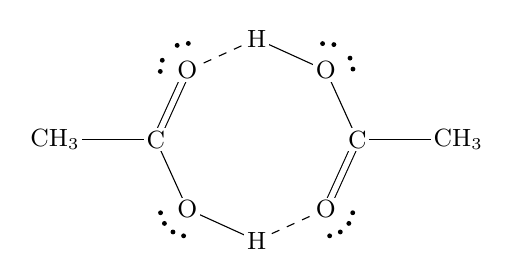
\begin{tikzpicture}[scale=0.8, every node/.style={font=\small}]
  \coordinate (Oa) at (-1.1, 1.1);
  \coordinate (C1) at (-1.6, 0);
  \coordinate (Ob) at (-1.1, -1.1);
  \coordinate (Hb) at (0, -1.6);
  \coordinate (Oc) at (1.1, -1.1);
  \coordinate (C2) at (1.6, 0);
  \coordinate (Od) at (1.1, 1.1);
  \coordinate (Hd) at (0, 1.6);
  \coordinate (Me1) at (-3.2, 0);
  \coordinate (Me2) at (3.2, 0);

  % ligações covalentes
  \draw[double, double distance=2pt] (C1) -- (Oa);
  \draw (C1) -- (Ob);
  \draw (Ob) -- (Hb);
  \draw (C1) -- (Me1);
  \draw[double, double distance=2pt] (C2) -- (Oc);
  \draw (C2) -- (Od);
  \draw (Od) -- (Hd);
  \draw (C2) -- (Me2);

  % pontes de hidrogênio (tracejadas)
  \draw[dashed] (Hb) -- (Oc);
  \draw[dashed] (Hd) -- (Oa);

  % pares de elétrons não ligantes (pontos), em coordenadas relativas ao O
  \begin{scope}[shift={(Oa)}]
    \foreach \a in {100,170} {
      \fill (\a:0.42) ++(\a+90:0.09) circle (1.1pt);
      \fill (\a:0.42) ++(\a-90:0.09) circle (1.1pt);
    }
  \end{scope}
  \begin{scope}[shift={(Ob)}]
    \foreach \a in {200,250} {
      \fill (\a:0.42) ++(\a+90:0.09) circle (1.1pt);
      \fill (\a:0.42) ++(\a-90:0.09) circle (1.1pt);
    }
  \end{scope}
  \begin{scope}[shift={(Oc)}]
    \foreach \a in {290,340} {
      \fill (\a:0.42) ++(\a+90:0.09) circle (1.1pt);
      \fill (\a:0.42) ++(\a-90:0.09) circle (1.1pt);
    }
  \end{scope}
  \begin{scope}[shift={(Od)}]
    \foreach \a in {15,85} {
      \fill (\a:0.42) ++(\a+90:0.09) circle (1.1pt);
      \fill (\a:0.42) ++(\a-90:0.09) circle (1.1pt);
    }
  \end{scope}

  % rótulos dos átomos
  \node[fill=white, inner sep=1pt] at (Oa) {$\mathrm{O}$};
  \node[fill=white, inner sep=1pt] at (Ob) {$\mathrm{O}$};
  \node[fill=white, inner sep=1pt] at (Oc) {$\mathrm{O}$};
  \node[fill=white, inner sep=1pt] at (Od) {$\mathrm{O}$};
  \node[fill=white, inner sep=1pt] at (C1) {$\mathrm{C}$};
  \node[fill=white, inner sep=1pt] at (C2) {$\mathrm{C}$};
  \node[fill=white, inner sep=1pt] at (Hb) {$\mathrm{H}$};
  \node[fill=white, inner sep=1pt] at (Hd) {$\mathrm{H}$};
  \node[fill=white, inner sep=1pt] at (Me1) {$\mathrm{CH_3}$};
  \node[fill=white, inner sep=1pt] at (Me2) {$\mathrm{CH_3}$};
\end{tikzpicture}
\end{center}
\begin{center}
\small Linhas contínuas: ligações covalentes; linhas tracejadas: pontes de hidrogênio; pontos: pares não ligantes.
\end{center}

\textbf{c)} Para $2\,\mathrm{M}\rightleftharpoons\mathrm{D}$:
\[
K_c=\frac{[\mathrm{D}]}{[\mathrm{M}]^2}.
\]
No equilíbrio, na base de 1 L: $[\mathrm{D}]=0{,}42\ \mathrm{mol\,L^{-1}}$ e $[\mathrm{M}]=1{,}00-2\times0{,}42=0{,}16\ \mathrm{mol\,L^{-1}}$. Conferência do balanço de massa: $[\mathrm{M}]+2[\mathrm{D}]=0{,}16+0{,}84=1{,}00\ \mathrm{mol\,L^{-1}}$. Logo
\[
K_c=\frac{0{,}42}{(0{,}16)^2}=\frac{0{,}42}{0{,}0256}\approx 16{,}4\ \mathrm{L\,mol^{-1}}.
\]
A unidade é $\mathrm{L\,mol^{-1}}$, pois $\Delta n=1-2=-1$. Como $K_c>1$ nessa base, o dímero é a espécie favorecida.

\textbf{d)} Dados: $c_0=0{,}10\ \mathrm{mol\,L^{-1}}$ de ácido acético (total analítico), com a mesma relação dímero/monômero do equilíbrio: $[\mathrm{D}]/[\mathrm{M}]=0{,}42/0{,}16=2{,}625$.

\begin{enumerate}
\item \textit{Concentrações.} Com $[\mathrm{M}]+2[\mathrm{D}]=c_0$ e $[\mathrm{D}]=2{,}625\,[\mathrm{M}]$, vem $[\mathrm{M}](1+5{,}25)=0{,}10$, logo $[\mathrm{M}]=0{,}016\ \mathrm{mol\,L^{-1}}$ e $[\mathrm{D}]=0{,}042\ \mathrm{mol\,L^{-1}}$. Equivalentemente, a fração de monômero associada é a mesma: 0,42 mol de dímero por mol inicial.

\item \textit{Fator de van't Hoff.} O abaixamento crioscópico depende do número de partículas dissolvidas. Por mol de ácido acético analítico:
\[
i=\frac{n_{\mathrm{M}}+n_{\mathrm{D}}}{n_0}=\frac{0{,}016+0{,}042}{0{,}10}=0{,}58.
\]
Confere com $i=1-0{,}42=0{,}58$: cada dímero consome 2 partículas e forma 1, ou seja, reduz o número de partículas em 1 por mol de dímero.

\item \textit{Molalidade.} Em 1 L de solução há $0{,}10$ mol de ácido acético, com massa $0{,}10\times60{,}05=6{,}005$ g, que ocupam $6{,}005/1{,}05=5{,}72$ mL (densidade $1{,}05\ \mathrm{kg\,L^{-1}}$). Admitindo volumes aditivos, o benzeno ocupa $1{,}000-0{,}006=0{,}994$ L, com massa $0{,}994\times0{,}87=0{,}865$ kg. Então
\[
W=\frac{0{,}10\ \mathrm{mol}}{0{,}865\ \mathrm{kg}}\approx 0{,}1156\ \mathrm{mol\,kg^{-1}}.
\]

\item \textit{Abaixamento crioscópico.} Com $K_f=5{,}12\ \mathrm{K\,kg\,mol^{-1}}$ (benzeno):
\[
\Delta T_f=i\,K_f\,W=0{,}58\times5{,}12\times0{,}1156\approx 0{,}343\ \mathrm{K}.
\]

\item \textit{Temperatura de fusão.}
\[
T_f=5{,}45-0{,}343\approx 5{,}11\ ^\circ\mathrm{C}.
\]
\end{enumerate}

\textit{Verificação.} Sem associação ($i=1$), seriam $\Delta T_f\approx0{,}59$ K e $T_f\approx4{,}86\ ^\circ\mathrm{C}$. A associação reduz o número de partículas e, portanto, o abaixamento, de modo que a solução congela cerca de 0,25 K mais perto do benzeno puro. A ordem de grandeza está coerente: $0{,}1\ \mathrm{mol\,kg^{-1}}\times5\ \mathrm{K\,kg\,mol^{-1}}\approx0{,}5$ K no caso ideal. Se o volume do soluto for desprezado ($W=0{,}10/0{,}87=0{,}115$ mol/kg), o resultado final continua $5{,}11\ ^\circ\mathrm{C}$.

\textit{Observação.} Não se reaproveita $K_c$ do item (c) neste caso: com $K_c$ fixo, a razão dímero/monômero mudaria com a diluição (em 0,10 mol/L daria $[\mathrm{D}]/[\mathrm{M}]\approx0{,}69$, e não $2{,}625$). O enunciado impõe a mesma relação, portanto a mesma fração associada.

ANSWER: a) ligações de hidrogênio (pontes $\mathrm{O{-}H\cdots O{=}C}$); b) dímero cíclico com duas pontes de hidrogênio, anel de 8 membros, $\mathrm{C_4H_8O_4}$ (ver figura); c) $K_c\approx16{,}4\ \mathrm{L\,mol^{-1}}$ (base de 1 mol/L); d) $T_f\approx5{,}11\ ^\circ\mathrm{C}$ ($\Delta T_f\approx0{,}34$ K, com $i=0{,}58$)%
\newpage%
\section*{Questão 5}

\section*{Solução}

\textbf{Hipóteses.} Além dos itens (i) a (v) do enunciado, adota-se:
\begin{itemize}
\item[(a)] Gases ideais, $PV=nRT$, com $R=8{,}3\,\text{J}\cdot\text{mol}^{-1}\cdot\text{K}^{-1}$, unidade compatível com a capacidade térmica dada em $\text{J}\cdot\text{K}^{-1}$.
\item[(b)] Hipótese de trabalho: a reação ocorre a $T=27+273=300\,\text{K}$, e a energia liberada é absorvida integralmente pelo calorímetro, de modo que o calor trocado vale $q=C\,\Delta T$. Assim, $\Delta U$ e $\Delta H$ são os valores da reação de 1,0 mol referidos a 300 K. O efeito do aquecimento dos produtos (correção de Kirchhoff) é desprezado.
\item[(c)] O calorímetro é adiabático e $C$ é constante no intervalo considerado.
\item[(d)] O único trabalho é o de expansão, $P\,\Delta V$.
\item[(e)] Hipótese (ii) vale para todas as espécies, inclusive $\text{O}_2$ (reagente) e $\text{H}_2\text{O}$ (produto).
\end{itemize}

\textbf{Passo 1: balanço de energia em cada calorímetro.} Como a combustão é exotérmica, o sistema cede calor ao calorímetro, e $\Delta T>0$ nos dois casos.

\emph{Volume constante.} Com $\Delta V=0$, o trabalho é nulo e a primeira lei dá $\Delta U=q_V$. O calorímetro absorve $C\,\Delta T_V$, logo $q_V=-C\,\Delta T_V$:
\[ \Delta U=-C\,\Delta T_V \]

\emph{Pressão constante.} Com $W=-P\,\Delta V$, a primeira lei dá $q_P=\Delta U+P\,\Delta V$. Como $P$ é constante, $P\,\Delta V=\Delta(PV)$, e portanto $q_P=\Delta(U+PV)=\Delta H$. Logo
\[ \Delta H=-C\,\Delta T_P \]

\textbf{Passo 2: relação entre $\Delta H$ e $\Delta U$.} Por definição, $\Delta H=\Delta U+\Delta(PV)$. Aplicando $PV=nRT$ a reagentes e produtos, à mesma temperatura,
\[ \Delta H-\Delta U=\Delta(PV)=\left(n_{\text{prod}}-n_{\text{reag}}\right)RT=\Delta n\,RT \]
em que $n$ são os mols de gás por mol de substância queimada e $\Delta n=n_{\text{prod}}-n_{\text{reag}}$.

\textbf{Passo 3: obtenção de $\Delta n$ a partir do item (v).} Subtraindo os resultados do Passo 1,
\[ \Delta H-\Delta U=-C\,\Delta T_P+C\,\Delta T_V=C\,(\Delta T_V-\Delta T_P) \]
O item (v) dá $\Delta T_V-\Delta T_P=16{,}6$ K, pois uma diferença de 16,6 $^{\circ}$C equivale a 16,6 K. (O mesmo número aparece na Folha de Dados como temperatura de fusão do ácido acético, mas aqui é apenas uma diferença de temperaturas.) Então
\[ \Delta H-\Delta U=450\times 16{,}6=7470\,\text{J}\cdot\text{mol}^{-1} \]
\[ \Delta n=\frac{\Delta H-\Delta U}{RT}=\frac{7470}{8{,}3\times 300}=\frac{7470}{2490}=3 \]

\emph{Unidades.} $C\,\Delta T$ é uma energia dividida por 1,0 mol, em J/mol, e $RT=2490\,\text{J}\cdot\text{mol}^{-1}$. Logo $\Delta n$ é adimensional. Os dados fornecem apenas a diferença $\Delta T_V-\Delta T_P$, de modo que $\Delta U$ e $\Delta H$ isoladamente não são determinados. A identificação não precisa deles.

\textbf{Passo 4: $\Delta n$ em função da fórmula.} Para a combustão completa de $\text{C}_x\text{H}_y$ gasoso,
\[ \text{C}_x\text{H}_y+\left(x+\frac{y}{4}\right)\text{O}_2\longrightarrow x\,\text{CO}_2+\frac{y}{2}\,\text{H}_2\text{O} \]
O balanço confere: C e H diretamente; para o O, $2\left(x+\frac{y}{4}\right)=2x+\frac{y}{2}$. Antes da reação há $1+x+\frac{y}{4}$ mol de gás, e depois há $x+\frac{y}{2}$ mol. Logo
\[ \Delta n=\left(x+\frac{y}{2}\right)-\left(1+x+\frac{y}{4}\right)=\frac{y}{4}-1 \]
resultado independente de $x$. Impondo $\Delta n=3$, obtém-se $y=16$.

\textbf{Passo 5: teste das quatro alternativas.} Pelo Passo 3, para cada substância,
\[ \Delta T_V-\Delta T_P=\frac{\Delta n\,RT}{C}=\frac{2490}{450}\,\Delta n\approx 5{,}53\,\Delta n\ \text{K} \]

\begin{center}
\begin{tabular}{lcccc}
\hline
Substância & $y$ & gases (reag. $\rightarrow$ prod.) & $\Delta n$ & $\Delta T_V-\Delta T_P$ (K) \\
\hline
acetileno ($\text{C}_2\text{H}_2$) & 2 & $3{,}5\rightarrow 3$ & $-\frac{1}{2}$ & $-2{,}77$ \\
p-xileno ($\text{C}_8\text{H}_{10}$) & 10 & $11{,}5\rightarrow 13$ & $\frac{3}{2}$ & $8{,}30$ \\
n-heptano ($\text{C}_7\text{H}_{16}$) & 16 & $12\rightarrow 15$ & $3$ & $16{,}6$ \\
propeno ($\text{C}_3\text{H}_6$) & 6 & $5{,}5\rightarrow 6$ & $\frac{1}{2}$ & $2{,}77$ \\
\hline
\end{tabular}
\end{center}

Só o n-heptano reproduz a diferença de 16,6 K. O acetileno daria $\Delta T_V<\Delta T_P$, contrariando (v). O p-xileno ($8{,}30$ K) e o propeno ($2{,}77$ K) dariam diferenças diferentes de 16,6 K.

\textbf{Verificação direta do n-heptano.}
\[ \text{C}_7\text{H}_{16}+11\,\text{O}_2\longrightarrow 7\,\text{CO}_2+8\,\text{H}_2\text{O} \]
Balanço: C: $7=7$; H: $16=2\cdot 8$; O: $2\cdot 11=14+8$. Os gases passam de $12$ para $15$ mol, logo $\Delta n=+3$.

\textbf{Conferência de sinais, casos particulares e ordens de grandeza.}
\begin{itemize}
\item \emph{Sinal.} Com $\Delta n=+3>0$, tem-se $\Delta H>\Delta U$ ($\Delta H$ é menos negativo), o que dá $\Delta T_V>\Delta T_P$, coerente com (v). Se os sinais de $q$ fossem trocados ($\Delta U=+C\,\Delta T_V$ e $\Delta H=+C\,\Delta T_P$), resultaria $\Delta n=-3$, que não coincide com nenhuma alternativa. O sinal adotado é, portanto, o consistente.
\item \emph{Casos particulares.} Se $\Delta n=0$ (por exemplo, eteno, $y=4$), os dois calorímetros se aquecem igualmente. Se $\Delta n<0$, a ordem se inverte, como no acetileno.
\item \emph{Ordem de grandeza.} $\Delta n\,RT\approx 7{,}5\,\text{kJ}\cdot\text{mol}^{-1}$. Frente a uma combustão típica de alcano, da ordem de $-4{,}8\,\text{MJ}\cdot\text{mol}^{-1}$, esse termo corresponde a cerca de $0{,}16\,\%$, coerente com um trabalho $P\,\Delta V$ pequeno. Os valores absolutos do enunciado são hipotéticos: uma energia de $4{,}8\,\text{MJ}$ elevaria $450\,\text{J}\cdot\text{K}^{-1}$ em cerca de $1{,}1\times 10^{4}$ K. Isso não afeta a identificação, que depende apenas da diferença.
\end{itemize}

\textbf{Conclusão.} Entre as quatro alternativas, só o n-heptano tem $\Delta n=+3$ (isto é, $y=16$) e reproduz $\Delta T_V-\Delta T_P=16{,}6$ K. A conclusão depende da premissa (ii), imposta pelo enunciado: se a água fosse líquida, nenhuma alternativa daria $\Delta n=+3$.

ANSWER: n-heptano ($\text{C}_7\text{H}_{16}$)%
\newpage%
\section*{Questão 6}

\section*{Solução}

\textbf{Hipóteses.} Além das condições do enunciado, adotam-se: (i) o equilíbrio ocorre apenas entre substâncias em fase líquida, sem equilíbrio líquido-vapor, e a mistura é homogênea; (ii) não há reações paralelas (por exemplo, a desidratação do etanol a éter etílico); (iii) o catalisador usual dessa reação, em geral um ácido forte como $\mathrm{H_2SO_4}$, altera a velocidade com que o equilíbrio é atingido, mas não a composição de equilíbrio nem o valor de $K_c$; (iv) $V$ constante, logo $[X]=n_X/V$; (v) $T$ e $p$ constantes, logo $K_c$ é constante; (vi) a atividade de cada espécie é aproximada pela concentração molar (mistura ideal), de modo que o $K_c$ obtido é um valor aparente, válido para essa mistura nessa temperatura. Os dados de benzeno, crioscopia e densidades da Folha de Dados não são necessários.

\textbf{a) Equação estequiométrica.} A reação é uma esterificação de Fischer (ácido carboxílico + álcool $\rightleftharpoons$ éster + água). Conservação dos átomos, com coeficientes $a,b,c,d$ para ácido, etanol, éster e água: C: $2a+2b=4c$; H: $4a+6b=8c+2d$; O: $2a+b=2c+d$. Resolvendo, obtém-se $d=a$, $b=a$ e $c=a$; logo a única solução com menores inteiros positivos é 1:1:1:1. Conferência com coeficientes unitários: C: $2+2=4$ e $4$; H: $4+6=8+2=10$; O: $2+1=2+1=3$. Assim:

\begin{align*}
\mathrm{CH_3COOH}\,(\ell) + \mathrm{C_2H_5OH}\,(\ell) \rightleftharpoons \mathrm{CH_3COOC_2H_5}\,(\ell) + \mathrm{H_2O}\,(\ell)
\end{align*}

\textbf{Quantidades iniciais.} Usam-se as massas molares da Tabela Periódica, $60{,}05$ e $46{,}07\ \text{g mol}^{-1}$, arredondadas para $60$ e $46\ \text{g mol}^{-1}$. O erro do arredondamento é inferior a $0{,}2\,\%$, bem abaixo da precisão do dado de $1{,}6$ mol, que tem dois algarismos significativos.

\begin{align*}
n_{\mathrm{ac},0} &= \frac{240\ \text{g}}{60\ \text{g mol}^{-1}} = 4{,}0\ \text{mol}, & n_{\mathrm{et},0} &= \frac{92\ \text{g}}{46\ \text{g mol}^{-1}} = 2{,}0\ \text{mol}
\end{align*}

Pela proporção 1:1, 4,0 mol de ácido consomem no máximo 2,0 mol de etanol. Logo o etanol é o reagente limitante e o ácido está em excesso. A conversão completa daria no máximo 2,0 mol de éster. O equilíbrio com 1,6 mol confirma reação incompleta, com etanol remanescente positivo.

\textbf{Quadro de equilíbrio.} Seja $x$ a quantidade (mol) de ácido e de etanol consumida. Pela estequiometria 1:1:1:1, a mesma quantidade é formada de éster e de água. No equilíbrio, $n_{\text{éster}}=n_{\mathrm{H_2O}}=1{,}6$ mol, logo $x_{\text{eq}}=1{,}6$ mol.

\begin{center}
\begin{tabular}{lccc}
\hline
Espécie & Início (mol) & Variação (mol) & Equilíbrio (mol)\\
\hline
$\mathrm{CH_3COOH}$ & $4{,}0$ & $-1{,}6$ & $2{,}4$\\
$\mathrm{C_2H_5OH}$ & $2{,}0$ & $-1{,}6$ & $0{,}4$\\
$\mathrm{CH_3COOC_2H_5}$ & $0$ & $+1{,}6$ & $1{,}6$\\
$\mathrm{H_2O}$ & $0$ & $+1{,}6$ & $1{,}6$\\
\hline
\end{tabular}
\end{center}

\textbf{b) Grau de equilíbrio do ácido acético.} Para um reagente, $\alpha=\dfrac{\text{quantidade reagida}}{\text{quantidade inicial}}$. Para o ácido, a referência é a quantidade inicial de ácido:

\begin{align*}
\alpha_{\mathrm{ac}} = \frac{1{,}6\ \text{mol}}{4{,}0\ \text{mol}} = 0{,}40 = 40\,\%
\end{align*}

Conferência: restam $2{,}4$ mol de ácido, e $2{,}4/4{,}0 = 0{,}60 = 1-\alpha$. O valor de $80\,\%$ ($1{,}6/2{,}0$) é o grau de conversão do etanol, o reagente limitante. Não é o valor pedido.

\textbf{c) Constante de equilíbrio.} Pela lei da ação das massas, com expoentes iguais aos coeficientes (todos iguais a 1) e a água no numerador:

\begin{align*}
K_c = \frac{[\mathrm{CH_3COOC_2H_5}]\,[\mathrm{H_2O}]}{[\mathrm{CH_3COOH}]\,[\mathrm{C_2H_5OH}]}
\end{align*}

Substituindo $[X]=n_X/V$:

\begin{align*}
K_c &= \frac{\dfrac{n_{\mathrm{es}}}{V}\cdot\dfrac{n_{\mathrm{H_2O}}}{V}}{\dfrac{n_{\mathrm{ac}}}{V}\cdot\dfrac{n_{\mathrm{et}}}{V}} = \frac{n_{\mathrm{es}}\,n_{\mathrm{H_2O}}}{n_{\mathrm{ac}}\,n_{\mathrm{et}}}\cdot\frac{V^{2}}{V^{2}} = \frac{n_{\mathrm{es}}\,n_{\mathrm{H_2O}}}{n_{\mathrm{ac}}\,n_{\mathrm{et}}}
\end{align*}

Pela relação geral $K_c=K_n\,V^{-\Delta n}$, com $\Delta n=(1+1)-(1+1)=0$, tem-se $K_c=K_n$, e o volume não influencia o resultado. Por isso a densidade do etanol, que não é dada, não é necessária. Como $\Delta n=0$, a unidade $(\text{mol}\,\text{L}^{-1})^{\Delta n}$ é igual a 1, e $K_c$ é adimensional. Substituindo os valores do quadro:

\begin{align*}
K_c = \frac{1{,}6\cdot 1{,}6}{2{,}4\cdot 0{,}4} = \frac{2{,}56}{0{,}96} = \frac{8}{3} \approx 2{,}67
\end{align*}

\textbf{Verificações.} (1) Com $x$ a extensão, $K_c=8/3$ dá $\dfrac{x^2}{(4{,}0-x)(2{,}0-x)}=\dfrac{8}{3}\Rightarrow 5x^2-48x+64=0\Rightarrow x=1{,}6$ ou $x=8{,}0$. Somente $x=1{,}6$ é aceitável, pois $x\le 2{,}0$ mol (limite imposto pelo etanol). (2) Com as massas molares da Tabela ($3{,}997$ e $1{,}997$ mol), obtém-se $K_c\approx 2{,}69$ e $\alpha\approx 40{,}0\,\%$. Os resultados coincidem a dois algarismos significativos, $K_c\approx 2{,}7$, compatível com o dado $1{,}6$ mol. (3) A prova não traz valor tabelado de $K_c$ para comparação, então a verificação é apenas interna.

ANSWER: a) $\mathrm{CH_3COOH}\,(\ell) + \mathrm{C_2H_5OH}\,(\ell) \rightleftharpoons \mathrm{CH_3COOC_2H_5}\,(\ell) + \mathrm{H_2O}\,(\ell)$ (coeficientes 1:1:1:1); b) $\alpha_{\mathrm{ac}} = 0{,}40 = 40\,\%$; c) $K_c = \dfrac{8}{3} \approx 2{,}7$ (adimensional)%
\newpage%
\section*{Questão 7}

\section*{Solução}

\textbf{Hipóteses.}
\begin{itemize}
\item (H1) Cada etapa é elementar, irreversível e obedece à lei de ação das massas: $r_{\mathrm{I}}=k_1[A][B]$, $r_{\mathrm{II}}=k_2[X][B]$, $r_{\mathrm{III}}=k_3[X][C]$.
\item (H2) Temperatura constante, logo $k_1$, $k_2$, $k_3$, $k$ e os expoentes são constantes; $[X]_0=0$.
\item (H3) $\nu_0$ é a velocidade inicial do regime quase estacionário: após um período de indução curto, $[X]$ atinge o valor estacionário (com $[X]\ll[A]_0,[B]_0,[C]_0$) e o consumo de A, B e C durante a medida é desprezível, de modo que se usam as concentrações iniciais. Em $t=0$ a lei prevê $\nu_P=0$, pois $[X]=0$; a grandeza medida é a taxa após a indução.
\item (H4) P se forma apenas na etapa II, com coeficiente 1: $\nu_P=\dfrac{d[P]}{dt}=r_{\mathrm{II}}$. Não vale $\nu_P=-\dfrac{d[A]}{dt}$ nem $\nu_P=-\dfrac{d[B]}{dt}$, pois $-\dfrac{d[A]}{dt}=r_{\mathrm{I}}$, $-\dfrac{d[B]}{dt}=r_{\mathrm{I}}+r_{\mathrm{II}}$, e X também é consumido na etapa III.
\end{itemize}

\textbf{Passo 1 (lei do mecanismo).} Pela aproximação do estado estacionário (AEE) para X,
\[ \frac{d[X]}{dt}=k_1[A][B]-k_2[X][B]-k_3[X][C]\approx0 \;\Rightarrow\; [X]=\frac{k_1[A][B]}{k_2[B]+k_3[C]}. \]
Substituindo em $\nu_0=k_2[X][B]$ e dividindo numerador e denominador por $k_3$:
\[ \nu_0=\frac{k_1k_2}{k_3}\,\frac{[A][B]^2}{[C]+\varepsilon[B]}, \qquad \varepsilon=\frac{k_2}{k_3}\ \ (\text{adimensional}). \]

\textbf{Passo 2 (o que os dados impõem a $\varepsilon$).} Experimento 2 frente ao 1: $[A][B]^2$ multiplica-se por $32$, e $[C]+\varepsilon[B]$ passa de $10^{-2}(1+\varepsilon)$ para $4\times10^{-2}(2+\varepsilon)$. Experimento 3 frente ao 1: $[A][B]^2$ multiplica-se por $16$, e $[C]+\varepsilon[B]$ passa para $2\times10^{-2}(8+\varepsilon)$. Logo
\[ \frac{\nu_{0,2}}{\nu_{0,1}}=\frac{8(1+\varepsilon)}{2+\varepsilon}=4 \qquad\text{e}\qquad \frac{\nu_{0,3}}{\nu_{0,1}}=\frac{8(1+\varepsilon)}{8+\varepsilon}=1, \]
e ambas exigem $\varepsilon=0$. Como as razões variam de $2\varepsilon$ e $0{,}875\,\varepsilon$ em torno de $\varepsilon=0$, a precisão de três algarismos impõe $|\varepsilon|\lesssim10^{-2}$. Assim $\varepsilon[B]/[C]\lesssim10^{-2}$ nos experimentos 1 a 3, e a lei de trabalho é
\[ \nu_0=\frac{k_1k_2}{k_3}\,\frac{[A][B]^2}{[C]}. \]

\textbf{Passo 3 (expoentes).} Razões em relação ao experimento 1:

Exp. 2/1: $[A]\times2$, $[B]\times4$, $[C]\times8$, $\nu_0\times4$, logo $2^{\alpha+2\beta+3\gamma}=2^{2}$:
\[ \alpha+2\beta+3\gamma=2 \qquad\text{(I)} \]
Exp. 3/1: $[A]\times4$, $[B]\times2$, $[C]\times16$, $\nu_0\times1$, logo $2^{2\alpha+\beta+4\gamma}=2^{0}$:
\[ 2\alpha+\beta+4\gamma=0 \qquad\text{(II)} \]
Exp. 4/1: $[A]\times8$, $[B]\times16$, $[C]\times2$:
\[ 3\alpha+4\beta+\gamma=\log_2\frac{\nu_{0,4}}{\nu_{0,1}} \qquad\text{(III)} \]

Como (I) e (II) são duas equações para três incógnitas, o mecanismo deve fechar o sistema. Nele, $\nu_0\propto[A]$ para qualquer $\varepsilon$, logo $\alpha=1$. Com $\alpha=1$, (I) e (II) viram $2\beta+3\gamma=1$ e $\beta+4\gamma=-2$, cuja solução é $\gamma=-1$, $\beta=2$. Conferência: (I) $1+4-3=2$; (II) $2+2-4=0$. Esta cadeia não usa o experimento 4.

\textbf{Passo 4 (verificação pelo experimento 4).} Com $(\alpha,\beta,\gamma)=(1,2,-1)$, a lei prevê $\nu_{0,4}/\nu_{0,1}=8\cdot16^2\cdot2^{-1}=1024$, ou seja $\nu_{0,4}=1{,}28\times10^{-3}\ \mathrm{mol\,L^{-1}\,s^{-1}}$. A equação (III) confere: $3+8-1=10=\log_2 1024$. O valor impresso é $1{,}28\times10^{-6}$. Com $\nu_{0,4}=1{,}28\times10^{-3}$, o sistema (I)–(III) tem determinante $20\neq0$ (coeficientes das linhas $(1,2,3)$, $(2,1,4)$, $(3,4,1)$) e solução única $(1,2,-1)$, sem uso do mecanismo.

\textbf{Hipótese (H5), a conferir na errata.} O expoente de $\nu_{0,4}$ está impresso com erro de potência de dez. Apoios: (i) a mantissa $1{,}28$ coincide com $1{,}25\times1{,}024$; (ii) os experimentos 1 a 3 são consistentes com a lei; (iii) a discrepância é exatamente $10^{3}$. Atribui-se o erro a $\nu_{0,4}$, e não às concentrações do experimento 4, porque a mantissa confere com a previsão.

\textbf{Se o valor impresso fosse tomado literalmente,} eliminando $\alpha$ entre (I) e (II) obtém-se $3\beta+2\gamma=4$; de (I), $\alpha=2-2\beta-3\gamma$; em (III), $2\beta+8\gamma=6-L$, com $L=\log_2 1{,}024$. Resolvendo,
\[ \gamma=\frac{10-3L}{20},\qquad \beta=\frac{4-2\gamma}{3},\qquad \alpha=2-2\beta-3\gamma. \]
Como $1{,}024=2^{7}/5^{3}$, $L=7-3\log_2 5\simeq0{,}0342$ (com $\ln2\simeq0{,}693$ e $\ln5\simeq1{,}609$ da Folha de Dados, $L\simeq0{,}035$), e então $\gamma\simeq0{,}49$, $\beta\simeq1{,}00$, $\alpha\simeq-1{,}49$. Exatamente, $\alpha=\dfrac{1-3\log_2 5}{4}$, $\beta=\dfrac{17-3\log_2 5}{10}$ e $\gamma=\dfrac{9\log_2 5-11}{20}$, todos irracionais, pois $\log_2 5=p/q$ levaria a $2^{p}=5^{q}$, impossível. Logo nenhuma lei com expoentes racionais reproduz o valor impresso. Os valores quase inteiros são uma armadilha: o terno $\left(-\tfrac{3}{2},1,\tfrac{1}{2}\right)$ satisfaz (I) e (II), mas daria razão $1$ no experimento 4, não $1{,}024$, e $\alpha=-\tfrac{3}{2}$ contradiz $\alpha=1$ do mecanismo. Portanto os itens a) a d) não dependem do valor impresso de $\nu_{0,4}$: usam (I), (II), o mecanismo e os experimentos 1 a 3. O experimento 4 serve só de checagem.

\textbf{Passo 5 (constante cinética).} Com $\alpha=1$, $\beta=2$, $\gamma=-1$, $k=\dfrac{\nu_{0,1}\,[C]_1}{[A]_1[B]_1^{2}}$:
\[ k=\frac{1{,}25\times10^{-6}\times10^{-2}}{10^{-2}\times10^{-4}}=1{,}25\times10^{-2}\ \mathrm{L\,mol^{-1}\,s^{-1}}. \]
Confirmação: experimento 2, $k=\dfrac{5{,}00\times10^{-6}\times8\times10^{-2}}{2\times10^{-2}\times(4\times10^{-2})^{2}}=1{,}25\times10^{-2}$; experimento 3, $k=\dfrac{1{,}25\times10^{-6}\times1{,}6\times10^{-1}}{4\times10^{-2}\times(2\times10^{-2})^{2}}=1{,}25\times10^{-2}$. Unidades: $\dfrac{(\mathrm{mol\,L^{-1}\,s^{-1}})(\mathrm{mol\,L^{-1}})}{(\mathrm{mol\,L^{-1}})^{3}}=\mathrm{L\,mol^{-1}\,s^{-1}}$. Também $k=k_1k_2/k_3$ tem essa unidade, pois cada $k_i$ é bimolecular.

\textbf{Respostas.}
\begin{itemize}
\item[a)] $\alpha=1$, $\beta=2$, $\gamma=-1$.
\item[b)] $k=1{,}25\times10^{-2}\ \mathrm{L\,mol^{-1}\,s^{-1}}$, com $k=k_1k_2/k_3$.
\item[c)] Lei completa, válida para qualquer $\varepsilon$:
\[ \nu_0=\frac{k_1k_2}{k_3}\,\frac{[A][B]^2}{[C]+\dfrac{k_2}{k_3}[B]}. \]
Na faixa dos dados, com $\dfrac{k_2}{k_3}[B]\ll[C]$ (verificado nos experimentos 1 a 3):
\[ \nu_0=1{,}25\times10^{-2}\,\frac{[A][B]^2}{[C]}\ \ \mathrm{mol\,L^{-1}\,s^{-1}}, \]
com concentrações em $\mathrm{mol\,L^{-1}}$ e $k$ em $\mathrm{L\,mol^{-1}\,s^{-1}}$.
\item[d)] $n=\alpha+\beta+\gamma=1+2-1=2$: reação de segunda ordem global (ordem 1 em A, 2 em B e $-1$ em C).
\end{itemize}

\textbf{Casos particulares e ordens de grandeza.}
\begin{itemize}
\item $\gamma<0$: aumentar $[C]$ reduz $\nu_0$, pois C consome X na etapa III, competindo com a etapa II. Isso é coerente com o mecanismo.
\item Limite $[C]\to0$: a lei simples diverge, mas a lei completa tende a $\nu_0\to k_1[A][B]$, finito e igual à taxa da etapa I (todo X passa a P). A lei simples só vale enquanto $\dfrac{k_2}{k_3}[B]\ll[C]$.
\item Ordem de grandeza: $1{,}25\times10^{-2}\cdot10^{-2}\cdot10^{-4}/10^{-2}=1{,}25\times10^{-6}\ \mathrm{mol\,L^{-1}\,s^{-1}}$, compatível com a tabela.
\end{itemize}

ANSWER: $\alpha=1$, $\beta=2$, $\gamma=-1$; $k=1{,}25\times10^{-2}\ \mathrm{L\,mol^{-1}\,s^{-1}}$; $\nu_0=1{,}25\times10^{-2}\,[A][B]^2/[C]$ (lei completa $\nu_0=\frac{k_1k_2}{k_3}\frac{[A][B]^2}{[C]+(k_2/k_3)[B]}$, válida para $(k_2/k_3)[B]\ll[C]$); ordem global $=2$. O valor $1{,}28\times10^{-6}$ do experimento 4 deve ser $1{,}28\times10^{-3}$ (hipótese a conferir na errata).%
\newpage%
\section*{Questão 8}

\section*{Solução}

\textbf{Passo 1 -- Reação e forma de Y.} Haletos de alquila reagem com sódio metálico em meio anidro pela \emph{reação de Wurtz}: dois grupos alquila se acoplam por uma ligação C--C. O meio deve ser anidro porque a água consumiria o sódio e o intermediário organometálico R--Na. Com 2 mol de RCl e 2 mol de Na (quantidade equivalente):

\[
2\,\mathrm{RCl} + 2\,\mathrm{Na} \longrightarrow \mathrm{R{-}R} + 2\,\mathrm{NaCl}
\]

Balanço: há 2 R, 2 Cl e 2 Na em cada lado. Como as duas metades de Y provêm do mesmo X, $Y = \mathrm{R{-}R}$ tem metades idênticas.

\emph{Hipótese:} ``alquila'' designa grupo saturado (radical de alcano), pois X é um cloreto de alquila. Essa hipótese garante a unicidade de X: sem ela, o 3-clorobut-1-eno daria o dímero 3,4-dimetil-hexa-1,5-dieno, também C$_8$ e meso, e o item (b) ficaria ambíguo.

\textbf{Passo 2 -- Condições sobre Y.}

\begin{itemize}
\item \emph{(i) Dois carbonos quirais.} Um carbono é quiral quando seus quatro ligantes são dois a dois distintos. Na reação, o Cl do carbono reativo é trocado pelo grupo R inteiro. Esse novo ligante é maior que qualquer ramo ligado ao mesmo carbono, logo continua distinto deles: nenhum centro surge nem desaparece. Assim, cada centro quiral de R reaparece em Y, uma vez em cada metade. Se R tem $n$ centros, $Y$ tem $2n$; de $2n = 2$ segue $n = 1$. Logo cada R tem exatamente um carbono quiral.

\item \emph{(ii) Opticamente inativo.} Pelo item (i), Y tem dois centros, C3 e C4 (numeração do hexano, Passo 3). Como as metades são idênticas, há três estereoisômeros: $(R,R)$, $(S,S)$ e $(R,S)$; $(S,R)$ é o mesmo composto que $(R,S)$, pois a numeração pode começar pelo outro lado.
\begin{itemize}
\item $(R,R)$ e $(S,S)$ são enantiômeros entre si. Cada um é quiral e desvia a luz, em sentidos opostos. A mistura 1:1 deles é inativa, mas são duas substâncias, e o enunciado fala de \emph{esse composto}.
\item $(R,S)$. Qualquer elemento de simetria imprópria (espelho, centro de inversão ou eixo $S_n$) de Y deve trocar C3 com C4. De fato, uma operação imprópria que deixasse C3 fixo fixaria seus quatro ligantes, que são distintos entre si; como esses quatro átomos não são coplanares, a operação seria a identidade. Como a operação troca C3 com C4 e inverte a configuração, C4 deve ter configuração oposta à de C3. Isso é compatível com $(R,S)$, não com $(R,R)$: se $(R,R)$ tivesse tal elemento, a imagem de C3 (R) seria um C4 de configuração S, contrariando C4 = R. Logo $(R,R)$ é quiral. Para $(R,S)$, a inversão no ponto médio de C3--C4 é de fato uma simetria (Passo 3): a molécula é aquiral, forma \emph{meso}, e não desvia a luz, pois as rotações de C3 e C4 se cancelam.
\end{itemize}
Logo $Y$ é o meso $(R,S)$, a única substância individual que cumpre (i) e (ii). C3 e C4 seguem sendo carbonos quirais na forma meso: o carbono é quiral por ter quatro ligantes distintos, e a molécula só é quiral se não tiver simetria imprópria. São coisas distintas.

\item \emph{(iii) Menor número de carbonos.} Se R tem $c$ carbonos, $Y$ tem $2c$. Testam-se as alquilas saturadas em ordem crescente de $c$:
\begin{itemize}
\item $c \le 3$: metila, etila, propila, isopropila e ciclopropila não têm centro quiral (isopropila tem dois CH$_3$ iguais; no anel da ciclopropila os dois CH$_2$ são equivalentes). Pelo item (i), Y não teria centro. Nenhuma serve.
\item $c = 4$: n-butila, isobutila e terc-butila não têm centro; os dímeros são octano, 2,5-dimetil-hexano e 2,2,3,3-tetrametil-butano, sem centro quiral. Entre as cíclicas, ciclobutila, ciclopropilmetila e 1-metilciclopropila também não têm centro. A 2-metilciclopropila tem dois (C1 e C2 do anel), o que daria $Y$ com quatro. Só a sec-butila, $\mathrm{CH_3CH_2CH(CH_3){-}}$, tem exatamente um.
\end{itemize}
Logo $R$ é a sec-butila e $Y$ tem 8 carbonos.
\end{itemize}

\textbf{Passo 3 -- Item (a): estrutura tridimensional de Y.} A cadeia principal é a mais longa, com seis carbonos (hexano). As metilas ficam em C3 e C4, com localizadores $\{3,4\}$ em qualquer sentido de numeração; logo Y é o 3,4-dimetil-hexano. Os centros quirais são C3 e C4. Prioridades CIP: em C3, C4 (C,C,H) $>$ C2 (C,H,H) $>$ CH$_3$ $>$ H; em C4, C3 $>$ C5 $>$ CH$_3$ $>$ H, pela simetria.

Desenho em zigue-zague no plano do papel, com C1 a C6:

\begin{center}
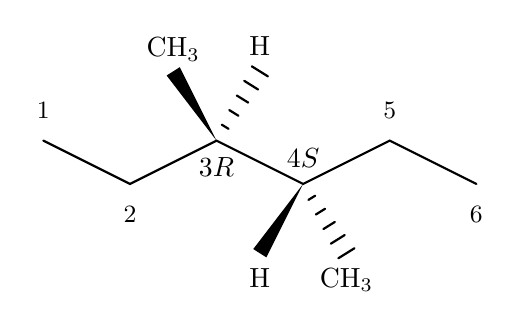
\begin{tikzpicture}[thick, line cap=round, scale=1.1]
  \draw (-1,0.5) -- (0,0) -- (1,0.5) -- (2,0) -- (3,0.5) -- (4,0);
  % C3: CH3 em cunha (para a frente), H tracejado (para trás)
  \fill (1,0.5) -- (0.424,1.252) -- (0.576,1.348) -- cycle;
  \draw (1.139,0.636) -- (1.061,0.684);
  \draw (1.253,0.787) -- (1.147,0.853);
  \draw (1.366,0.939) -- (1.234,1.021);
  \draw (1.480,1.090) -- (1.320,1.190);
  \draw (1.593,1.242) -- (1.407,1.358);
  \node[above] at (0.5,1.3) {$\mathrm{CH_3}$};
  \node[above] at (1.5,1.36) {$\mathrm{H}$};
  % C4: CH3 tracejada (para trás), H em cunha (para a frente)
  \draw (2.061,-0.184) -- (2.139,-0.136);
  \draw (2.147,-0.353) -- (2.253,-0.287);
  \draw (2.234,-0.521) -- (2.366,-0.439);
  \draw (2.320,-0.690) -- (2.480,-0.590);
  \draw (2.407,-0.858) -- (2.593,-0.742);
  \node[below] at (2.5,-0.86) {$\mathrm{CH_3}$};
  \fill (2,0) -- (1.576,-0.848) -- (1.424,-0.752) -- cycle;
  \node[below] at (1.5,-0.86) {$\mathrm{H}$};
  \node at (1,0.2) {$3R$};
  \node at (2,0.3) {$4S$};
  \node[font=\small] at (-1,0.85) {$1$};
  \node[font=\small] at (0,-0.35) {$2$};
  \node[font=\small] at (3,0.85) {$5$};
  \node[font=\small] at (4,-0.35) {$6$};
\end{tikzpicture}
\end{center}

Verificação:
\begin{itemize}
\item \emph{C3:} H tracejado (para trás). A sequência C4 $\to$ C2 $\to$ CH$_3$ é horária no plano; com o H para trás, a configuração é $R$.
\item \emph{C4:} H em cunha (para a frente). A sequência C3 $\to$ C5 $\to$ CH$_3$ é horária no plano, mas o H aponta para o observador, o que inverte o sentido: $S$.
\item \emph{Forma meso:} a inversão no ponto médio de C3--C4 leva C1 em C6, C2 em C5, C3 em C4, a metila em cunha de C3 na metila tracejada de C4 e o H tracejado de C3 no H em cunha de C4. A molécula coincide com sua imagem, logo é aquiral. Se as duas metilas estivessem em cunha, o resultado seria $(3R,4R)$, quiral, o que contraria (ii).
\end{itemize}

Logo $Y$ é o $(3R,4S)$-3,4-dimetil-hexano, forma meso.

\textbf{Passo 4 -- Item (b): nome IUPAC de X.} X é o haleto que origina a sec-butila: $\mathrm{CH_3CH_2CHClCH_3}$. A cadeia principal tem quatro carbonos (butano) e o Cl está em C2; numerada pelo outro lado, o Cl ficaria em C3, e vale o menor localizador. Logo X é o \textbf{2-clorobutano} (cloreto de sec-butila). Entre os isômeros $\mathrm{C_4H_9Cl}$, só ele tem centro quiral: 1-clorobutano, 1-cloro-2-metilpropano e 2-cloro-2-metilpropano não têm.

\emph{Racemato.} Para formar o meso, um fragmento (R) precisa se unir a um fragmento (S). Logo X fornece os dois enantiômeros, isto é, X é o (RS)-2-clorobutano. Se X fosse enantiomericamente puro, Y seria (R,R) ou (S,S), opticamente ativo. Como ilustração, e não como premissa do enunciado, um acoplamento sem estereosseletividade daria na mistura bruta 50\% de meso e 50\% de dl. O enunciado, porém, trata Y como composto único e inativo, o que identifica a forma meso.

\textbf{Conferência.} A equação de Wurtz fecha (2 Cl e 2 Na em cada lado); Y é C$_8$H$_{18}$, com dois centros e forma meso; X é o único isômero de C$_4$H$_9$Cl com centro quiral.

ANSWER: a) $(3R,4S)$-3,4-dimetil-hexano (forma meso, $\mathrm{C_8H_{18}}$), em zigue-zague com a metila de C3 em cunha, o H de C3 tracejado, a metila de C4 tracejada e o H de C4 em cunha; b) 2-clorobutano (cloreto de sec-butila), $\mathrm{CH_3CH_2CHClCH_3}$, usado como racemato (RS).%
\newpage%
\section*{Questão 9}

\section*{Solução}

\textbf{Hipóteses.}
\begin{itemize}
\item[H1] Solução diluída e ideal: $\Delta T_f=i\,K_f\,b$, com $b$ a molalidade (mol de soluto por kg de solvente) e $K_f=5{,}12\ \mathrm{K\,kg\,mol^{-1}}$.
\item[H2] No equilíbrio sólido-líquido, o sólido que se separa é benzeno puro; o soluto não entra na rede cristalina.
\item[H3] $i=1$: A não se dissocia nem se associa em benzeno. O enunciado não fornece constante de associação, então uma associação parcial não pode ser quantificada; $i=1$ é a hipótese que torna o problema determinado.
\item[H4] "Composto aromático" significa derivado do benzeno, com anel aromático de seis carbonos. Assim, tropona, heteroaromáticos e compostos não aromáticos ficam excluídos.
\item[H5] "Halogenação" significa monossubstituição no anel por substituição eletrofílica aromática, $\mathrm{C_8H_{10}+X_2\rightarrow C_8H_9X+HX}$, com $\mathrm{FeX_3}$ como catalisador. A justificativa está no Passo 5.
\end{itemize}

\textbf{Dados não usados.} A densidade do benzeno, pois a lei usa massa de solvente (dividir $2$ kg por $0{,}87\ \mathrm{kg\,L^{-1}}$ daria um volume, erro a evitar). $R$, $\ln 2$ e $\ln 5$ pertencem a gases, cinética e equilíbrio. $K_f$ e o ponto de fusão do ácido acético referem-se a outro solvente. O ponto de fusão do benzeno é dispensável, pois $\Delta T_f$ já é dado.

\textbf{Passo 1: massa molar de A.} Com $i=1$ e $b=\dfrac{m_A}{M_A\,m_{\mathrm{solv}}}$, a lei crioscópica fornece
\[
M_A=\frac{K_f\,m_A}{\Delta T_f\,m_{\mathrm{solv}}}.
\]
Com $\Delta T_f=1{,}28$ K (a mesma variação em kelvin e em graus Celsius), $m_A=53$ g e $m_{\mathrm{solv}}=2$ kg:
\[
M_A=\frac{5{,}12\times 53}{1{,}28\times 2}\ \mathrm{g\,mol^{-1}}=\frac{271{,}36}{2{,}56}\ \mathrm{g\,mol^{-1}}=106\ \mathrm{g\,mol^{-1}}.
\]
Unidades: $\mathrm{K\,kg\,mol^{-1}}\cdot\mathrm{g}/(\mathrm{K\,kg})=\mathrm{g\,mol^{-1}}$.

\textbf{Verificação.} $n_A=53/106=0{,}50$ mol, $b=0{,}50/2=0{,}25$ mol/kg e $K_f\,b=5{,}12\times 0{,}25=1{,}28$ K, que é o valor dado. A ordem de grandeza é compatível com aromáticos pequenos (benzeno, 78 g/mol; tolueno, 92 g/mol).

\textbf{Sobre H3.} Se A dimerizasse por completo ($i=\tfrac{1}{2}$), a massa molar do monômero seria $53$ g/mol, abaixo de $78$ g/mol, a massa do próprio benzeno. Um derivado benzênico não pode ter essa massa, logo a dimerização total é excluída. Associações parciais não são excluídas por esse cálculo; ficam fora pela hipótese H3.

\textbf{Passo 2: estruturas benzênicas com $105\leq M\leq 107$.} Os dados têm dois ou três algarismos significativos ($53$ g; $1{,}28\ ^\circ$C), logo $M$ é conhecida a cerca de $\pm 1$ g/mol. Usam-se massas nominais (C 12, H 1, N 14, O 16) e a janela $105\leq M\leq 107$. Um derivado benzênico é $\mathrm{C_6H_6}$ (78 g/mol) com $k$ hidrogênios substituídos por grupos monovalentes de massas $m_i$:
\[
M=78+\sum_{i=1}^{k}(m_i-1).
\]
Portanto $\sum(m_i-1)$ deve ficar entre 27 e 29.
\begin{itemize}
\item \textit{Número de substituintes.} O grupo mais leve é $\mathrm{CH_3}$ (15 g/mol), que contribui com 14. Com $k=3$, $M\geq 78+42=120$; logo $k\leq 2$.
\item \textit{Anel isolado.} Um anel fundido ao benzeno exigiria pelo menos $\mathrm{C_9}$ (108 g/mol); logo não há anel fundido.
\item \textit{Caso $k=1$.} Enumerando sistematicamente fórmulas $\mathrm{C_aH_bN_cO_dF_e}$ de camada fechada (paridade e DBE inteiro e não negativo), os grupos de massa 28, 29 ou 30 são: $\mathrm{CH{=}NH}$ e $\mathrm{N{=}CH_2}$ (28); $\mathrm{CHO}$, $\mathrm{C_2H_5}$ e $\mathrm{N{=}NH}$ (29); $\mathrm{NO}$, $\mathrm{CH_2NH_2}$ e $\mathrm{NHCH_3}$ (30). Grupos com P, S, Cl ou F não aparecem nessa faixa.
\item \textit{Caso $k=2$.} A soma $m_1+m_2$ deve ficar entre 29 e 31. Como o outro grupo tem massa de pelo menos 15, cada grupo tem massa no máximo 16. Os únicos grupos de camada fechada com essa massa são $\mathrm{CH_3}$ (15) e $\mathrm{NH_2}$ (16). Assim, $\mathrm{CH_3}+\mathrm{CH_3}$ dá $M=106$, $\mathrm{CH_3}+\mathrm{NH_2}$ dá $M=107$, e $\mathrm{NH_2}+\mathrm{NH_2}$ dá 108, fora da janela. Isso também exclui F, P, S e Cl com $k=2$.
\end{itemize}

Candidatos resultantes:
\begin{center}
\begin{tabular}{lll}
Fórmula & Estruturas benzênicas & $M$ (g/mol) \\
\hline
$\mathrm{C_7H_7N}$ & $\mathrm{C_6H_5CH{=}NH}$; $\mathrm{C_6H_5N{=}CH_2}$ & 105 \\
$\mathrm{C_7H_6O}$ & $\mathrm{C_6H_5CHO}$ & 106 \\
$\mathrm{C_6H_6N_2}$ & $\mathrm{C_6H_5N{=}NH}$ & 106 \\
$\mathrm{C_8H_{10}}$ & $\mathrm{C_6H_5CH_2CH_3}$; o-, m- e p-xileno & 106 \\
$\mathrm{C_6H_5NO}$ & nitrosobenzeno & 107 \\
$\mathrm{C_7H_9N}$ & $\mathrm{C_6H_5CH_2NH_2}$; $\mathrm{C_6H_5NHCH_3}$; o-, m- e p-toluidina & 107 \\
\end{tabular}
\end{center}

\textbf{Passo 3: eliminação.}
\begin{itemize}
\item \textit{Tollens.} O reagente oxida aldeídos a carboxilatos, reduzindo $\mathrm{Ag^+}$ a espelho de prata:
\[
\mathrm{RCHO}+2\,[\mathrm{Ag(NH_3)_2}]^{+}+3\,\mathrm{OH^-}\rightarrow \mathrm{RCOO^-}+2\,\mathrm{Ag}\!\downarrow+4\,\mathrm{NH_3}+2\,\mathrm{H_2O}
\]
O benzaldeído daria espelho, logo é excluído. Os demais candidatos não têm CHO, e o teste é negativo para eles, então não os distingue.
\item \textit{Instabilidade.} $\mathrm{C_6H_5CH{=}NH}$ e $\mathrm{C_6H_5N{=}CH_2}$ são iminas que hidrolisam; $\mathrm{C_6H_5N{=}NH}$ se decompõe em benzeno e $\mathrm{N_2}$. Não são compostos estáveis e não podem ser A.
\item \textit{Halogenação no anel.} Cada classe de hidrogênios não equivalentes por simetria gera um produto distinto:
\end{itemize}
\begin{center}
\begin{tabular}{llc}
Composto & Classes de H no anel & Produtos no anel \\
\hline
$\mathrm{C_6H_5CH_2CH_3}$ & o, m, p & 3 \\
$\mathrm{C_6H_5NO}$ & o, m, p & 3 \\
$\mathrm{C_6H_5CH_2NH_2}$ & o, m, p & 3 \\
$\mathrm{C_6H_5NHCH_3}$ & o, p & 2 (além da N-halogenação) \\
o-toluidina & 3, 4, 5, 6 & 4 \\
m-toluidina & 2, 4, 5, 6 & 4 \\
p-toluidina & $2\equiv 6$; $3\equiv 5$ & 2 \\
o-xileno & $3\equiv 6$; $4\equiv 5$ & 2 \\
m-xileno & $2$; $4\equiv 6$; $5$ & 3 \\
p-xileno & $2\equiv 3\equiv 5\equiv 6$ & 1 \\
\end{tabular}
\end{center}
No etilbenzeno, a cadeia lateral daria ainda $\mathrm{C_6H_5CH(X)CH_3}$ e $\mathrm{C_6H_5CH_2CH_2X}$, mais um motivo para a exclusão.

\textbf{Passo 4: conclusão.} Só o p-xileno (1,4-dimetilbenzeno) tem uma única classe de hidrogênio no anel. Sua monohalogenação gera um único produto, o 2-X-1,4-dimetilbenzeno, com X = Cl ou Br. Confere a massa: $\mathrm{C_6H_4(CH_3)_2}$ tem $8\times 12+10=106$ g/mol.
% Pré-requisito no preâmbulo: \usepackage{tikz}
\begin{center}
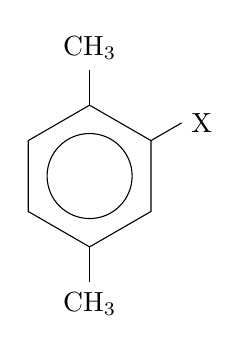
\begin{tikzpicture}[scale=0.9]
  \coordinate (a) at (90:1);
  \coordinate (b) at (30:1);
  \coordinate (c) at (-30:1);
  \coordinate (d) at (-90:1);
  \coordinate (e) at (-150:1);
  \coordinate (f) at (150:1);
  \draw (a)--(b)--(c)--(d)--(e)--(f)--cycle;
  \draw (0,0) circle (0.6);
  \draw (a)--++(90:0.5) node[above] {$\mathrm{CH_3}$};
  \draw (d)--++(-90:0.5) node[below] {$\mathrm{CH_3}$};
  \draw (b)--++(30:0.5) node[right] {$\mathrm{X}$};
\end{tikzpicture}
\end{center}

\textbf{Passo 5: justificativa de H5.} Se a halogenação fosse radicalar na cadeia lateral, cada xileno daria um único $\mathrm{ArCH_2X}$, pois os dois $\mathrm{CH_3}$ são equivalentes em cada isômero. Então o enunciado não distinguiria o-, m- e p-xileno, o que contraria a existência de uma resposta única. Logo a leitura pretendida é a substituição eletrofílica no anel. Nessa leitura radicalar, o etilbenzeno ainda seria excluído, pois daria dois produtos possíveis ($\mathrm{C_6H_5CH(X)CH_3}$ e $\mathrm{C_6H_5CH_2CH_2X}$). Por fim, "único produto" refere-se à monossubstituição: com excesso de $\mathrm{X_2}$, o p-xileno daria produtos di-, tri- e tetra-halogenados.

ANSWER: A é o p-xileno (1,4-dimetilbenzeno), $\mathrm{C_8H_{10}}$, com $M=106\ \mathrm{g\,mol^{-1}}$; sua monohalogenação no anel gera um único produto, o 2-X-1,4-dimetilbenzeno.%
\newpage%
\section*{Questão 10}

\section*{Solução}

\textbf{Hipóteses.}
\begin{itemize}
\item Sistema fechado desde a formação do mineral: nenhum ${}^{232}\mathrm{Th}$, ${}^{208}\mathrm{Pb}$ ou intermediário entra ou sai, incluindo o gás ${}^{220}\mathrm{Rn}$. Um escape de radônio faria o chumbo medido ser menor e a idade ser subestimada.
\item Chumbo inicial nulo: todo o ${}^{208}\mathrm{Pb}$ é radiogênico, logo $N_{\mathrm{Pb}}(0)=0$.
\item Decaimento de primeira ordem, com $\lambda$ constante.
\item A razão molar $0{,}024$ é igual à razão entre números de átomos, pois $N_{\mathrm{A}}$ se cancela.
\end{itemize}

\textbf{Passo 1 -- Estequiometria da cadeia.} Sejam $x$ emissões $\alpha$ e $y$ emissões $\beta^-$ entre ${}^{232}\mathrm{Th}$ e ${}^{208}\mathrm{Pb}$. A emissão $\alpha$ reduz $A$ em $4$ e $Z$ em $2$; a emissão $\beta^-$ mantém $A$ e aumenta $Z$ em $1$. Logo
\[
4x=232-208=24,\qquad 2x-y=90-82=8,
\]
donde $x=6$ e $y=4$. Cada ${}^{232}\mathrm{Th}$ desintegrado produz, no fim da cadeia, exatamente um ${}^{208}\mathrm{Pb}$. Os ramos alternativos, como o do ${}^{212}\mathrm{Bi}$, têm o mesmo balanço líquido.

\textbf{Passo 2 -- Intermediários desprezíveis.} As meias-vidas dos intermediários vão de $0{,}3\,\mu\mathrm{s}$ (${}^{212}\mathrm{Po}$) a $5{,}75$ anos (${}^{228}\mathrm{Ra}$), muito menores que $T_{\mathrm{Th}}$. Para $t\gg T_i$ (aqui $t\approx5\times10^{8}$ anos $\gg5{,}75$ anos), cada intermediário já atingiu o equilíbrio com o pai, com atividades iguais, $\lambda_iN_i=\lambda_{\mathrm{Th}}N_{\mathrm{Th}}$, logo $N_i\approx(T_i/T_{\mathrm{Th}})\,N_{\mathrm{Th}}$. Como $T_{\mathrm{Th}}\gg T_i$, o pai quase não varia nesse intervalo. Somando,
\[
\sum_i N_i\approx\frac{\sum_i T_i}{T_{\mathrm{Th}}}\,N_{\mathrm{Th}}\approx\frac{7{,}7}{1{,}41\times10^{10}}\,N_{\mathrm{Th}}\approx5\times10^{-10}\,N_{\mathrm{Th}}.
\]
Frente ao chumbo formado, que corresponde a cerca de $2{,}3\%$ do tório original, essa soma é desprezível (erro relativo da ordem de $10^{-8}$).

\textbf{Passo 3 -- Lei do decaimento e balanço de átomos.} Para o tório,
\[
N_{\mathrm{Th}}(t)=N_{\mathrm{Th}}(0)\,e^{-\lambda t},\qquad \lambda=\frac{\ln 2}{T_{\mathrm{Th}}},
\]
pois $N(T_{\mathrm{Th}})=N(0)/2$ implica $e^{-\lambda T_{\mathrm{Th}}}=\tfrac12$. Pela conservação de átomos, desprezando os intermediários,
\[
N_{\mathrm{Pb}}(t)=N_{\mathrm{Th}}(0)-N_{\mathrm{Th}}(t)=N_{\mathrm{Th}}(t)\left(e^{\lambda t}-1\right).
\]
Dividindo por $N_{\mathrm{Th}}(t)$, o tório presente hoje, a razão medida é
\[
R=\frac{N_{\mathrm{Pb}}(t)}{N_{\mathrm{Th}}(t)}=e^{\lambda t}-1=0{,}024\quad\Longrightarrow\quad e^{\lambda t}=1{,}024.
\]

\textbf{Passo 4 -- Isolamento de $t$.} Tomando o logaritmo natural e usando $\lambda=\ln 2/T_{\mathrm{Th}}$,
\[
t=\frac{\ln(1{,}024)}{\lambda}=\frac{T_{\mathrm{Th}}}{\ln 2}\,\ln(1+R).
\]

\textbf{Passo 5 -- Cálculo.} Primeiro, $\dfrac{T_{\mathrm{Th}}}{\ln 2}=\dfrac{1{,}41\times10^{10}}{0{,}693}\approx2{,}035\times10^{10}$ anos.

\emph{Valor exato.} $\ln(1{,}024)=0{,}02372$, obtido pela série $R-\tfrac{R^2}{2}+\tfrac{R^3}{3}-\dots$ com $R=0{,}024$. Logo
\[
t=2{,}035\times10^{10}\times0{,}02372\approx4{,}83\times10^{8}\ \text{anos}.
\]

\emph{Aproximação com a Folha de Dados.} Como $1{,}024=2^{7}/5^{3}$,
\[
\ln(1{,}024)=7\ln2-3\ln5\approx7(0{,}693)-3(1{,}609)=0{,}024.
\]
Esse $0{,}024$ coincide com $R$ apenas por arredondamento dos logaritmos, pois o valor exato é $0{,}02372$. Com a linearização $e^{\lambda t}-1\approx\lambda t$, válida porque $\lambda t\approx0{,}024\ll1$, obtém-se
\[
t\approx2{,}035\times10^{10}\times0{,}024\approx4{,}88\times10^{8}\ \text{anos}.
\]

\emph{Precisão.} $R$ tem dois algarismos significativos, logo $0{,}0235\le R\le0{,}0245$ e a idade fica entre $4{,}7$ e $4{,}9\times10^{8}$ anos, com incerteza de cerca de $\pm2\%$. Os dois cálculos caem nessa faixa: o exato dá $4{,}8\times10^{8}$ anos e a linearização dá $4{,}9\times10^{8}$ anos.

\textbf{Passo 6 -- Verificação.}
\begin{itemize}
\item \textit{Unidades e reconstituição}: $\lambda=\dfrac{0{,}693}{1{,}41\times10^{10}}\approx4{,}9\times10^{-11}\ \text{ano}^{-1}$, e $\lambda t\approx4{,}9\times10^{-11}\times4{,}83\times10^{8}\approx0{,}024$ é adimensional. Além disso, $e^{0{,}02372}=1{,}0240$, que reproduz a razão medida.
\item \textit{Erro da linearização}: $e^{\lambda t}-1\approx\lambda t$ superestima $\lambda t$ em $R-\ln(1+R)\approx R^2/2$. Isso dá um erro relativo de $R/2\approx1{,}2\%$ na idade, que explica a diferença entre $4{,}88$ e $4{,}83$.
\item \textit{Ordem de grandeza}: $t\approx5\times10^{8}$ anos $\ll T_{\mathrm{Th}}=1{,}41\times10^{10}$ anos, e a fração de tório decaída é $R/(1+R)\approx2{,}3\%$, coerente com $\lambda t\ll1$. Como $R>0$, resulta $t>0$.
\end{itemize}

\textbf{Armadilhas e consequências numéricas.}
\begin{itemize}
\item Esquecer o $-1$ e usar $e^{\lambda t}=R$: $t=\dfrac{T_{\mathrm{Th}}}{\ln2}\ln(0{,}024)\approx-7{,}6\times10^{10}$ anos, negativo e impossível.
\item Inverter a razão, com $e^{\lambda t}=1+1/R\approx42{,}7$: $t\approx7{,}6\times10^{10}$ anos, cerca de cinco meias-vidas do tório, incompatível com a pequena fração decaída.
\item Usar $T_{1/2}({}^{238}\mathrm{U})$ no lugar do tório: $t\approx1{,}5\times10^{8}$ anos, cerca de um terço do valor correto.
\item Esquecer $\ln 2$, com $t=T_{\mathrm{Th}}\ln(1+R)$: $t\approx3{,}3\times10^{8}$ anos, cerca de $30\%$ abaixo.
\item Os percentuais de $\mathrm{ThO}_2$ e $\mathrm{U}_3\mathrm{O}_8$, as massas molares e as densidades não entram. A razão Th/U atual não fornece idade sem a razão ${}^{206}\mathrm{Pb}/{}^{238}\mathrm{U}$, que não foi dada.
\end{itemize}

\noindent ANSWER: $t\approx4{,}8\times10^{8}$ a $4{,}9\times10^{8}$ anos (ordem de $5\times10^{8}$ anos)%
\newpage%
\section*{Apêndice: parecer do avaliador}%
\subsection*{Questão 1: nota 9,0 (aprovada, rodada 3 de 3)}%
\textbf{Resposta da resolução às cegas do avaliador:} Massa de MnO2 necessária: 0,87 g ($\approx$ 0,010 mol de MnO2).\newline%
\newline%
Reações: MnO2 + 4 HCl $\to$ MnCl2 + Cl2 + 2 H2O; Cl2 + 2 NaBr $\to$ 2 NaCl + Br2; global: MnO2 + 4 HCl + 2 NaBr $\to$ MnCl2 + 2 NaCl + Br2 + 2 H2O.\newline%
\newline%
Cálculo: n(NaBr) = 2,06/103 = 0,0200 mol $\to$ n(Cl2) = 0,0100 mol $\to$ n(MnO2) = 0,0100 mol $\to$ m = 0,87 g.\newline%
\newline%
Não há alternativas de múltipla escolha nesta questão.\par %
Resposta final conferida: a resolução do candidato dá m(MnO2) $\approx$ 0,870 g, o mesmo resultado da referência (0,87 g). A diferença está só no número de algarismos significativos, e 0,870 g é defensável porque 2,06 g tem três algarismos. Verifiquei o enunciado no PDF e recalculei tudo com python: n(NaBr) = 0,020021 mol, n(MnO2) = n(Cl2) = 0,010010 mol, m = 0,87026 g. A checagem do bromo dá 1,5997 g de Br2 para 1,5997 g de Br na amostra. Os erros comuns citados também batem: 1:1 daria 1,74 g e 2 Cl2 por MnO2 daria 0,435 g. Os valores de massa molar que o candidato atribui à tabela periódica da prova (Na 22,990; Br 79,904; Mn 54,938; O 15,999) estão corretos, conferidos na ampliação da página 1. Minha referência dizia que a tabela traz valores inteiros (Na = 23, Br = 80 etc.); isso estava errado, e o candidato citou a tabela de forma mais precisa. Todas as armadilhas da referência foram tratadas: razão 1:2 NaBr:Cl2, razão 1:1 MnO2:Cl2, 4 HCl por Cl2, MnO2 puro e não minério, distratores da Folha de Dados, papel redox com semirreações, unidades e algarismos significativos. As reações estão balanceadas e verificadas por átomos e por elétrons. Os problemas que restam são de redação e concisão, sem erro de conta ou de conceito, por isso a nota é 9. Com as correções das hipóteses (ii) e (iii), a resolução poderia sair como gabarito comentado."\}{]}%
\begin{itemize}%
\item%
{[}minor{]} Hipótese (ii) está mal redigida: a frase "não ser reagente não implica estar em excesso" é confusa. O correto seria dizer que o enunciado não informa a quantidade de HCl, então a suficiência é uma premissa assumida, e não uma conclusão. Reescrever a hipótese nesses termos.%
\item%
{[}minor{]} Hipótese (iii) é imprecisa: afirma que o excesso de Cl2 "alteraria a relação 2 NaBr : 1 Cl2". O excesso de Cl2 não muda a estequiometria da liberação; ele consome parte do Br2 (via BrCl), o que reduziria a recuperação de bromo e exigiria mais Cl2. Reformular a frase nesse sentido.%
\item%
{[}minor{]} O enunciado pede HCl concentrado, mas a resolução não explica por que a concentração importa para a reação. Uma observação curta bastaria: o HCl diluído não gera Cl2 em quantidade significativa com MnO2. Isso justificaria a hipótese (ii) sem depender só de suposição.%
\item%
{[}minor{]} A resolução é longa para uma questão de 1,0 ponto. Há cinco hipóteses, três blocos de conferência e vários erros comuns repetidos. Nada está errado, mas um gabarito enxuto poderia manter só as hipóteses essenciais (rendimento, Cl2 mínimo, Br totalmente na forma Br$^{-}$, MnO2 puro) e a checagem do balanço de bromo.%
\end{itemize}%
\subsection*{Questão 2: nota 9,0 (aprovada, rodada 2 de 2)}%
\textbf{Resposta da resolução às cegas do avaliador:} a) Gráfico P $\times$ V: ciclo fechado 1$\to$2$\to$3$\to$4$\to$1, percorrido no sentido horário no plano (V, P).\newline%
{-} Etapa I: isoterma a T1, sólida, de 1 (V1, P1) para 2 (V2 < V1, P2 > P1). É compressão.\newline%
{-} Etapa II: compressão rápida e irreversível, de 2 para 3, tracejada. V3 < V2, P3 > P2, T3 > T1.\newline%
{-} Etapa III: isoterma a T3 > T1, sólida, de 3 para 4 (V4 > V3, P4 < P3). É expansão.\newline%
{-} Etapa IV: expansão rápida e irreversível, de 4 para 1, tracejada. V1 > V4, P1 < P4, T cai de T3 para T1.\newline%
{-} Ordens: V3 < V2 < V1 e V3 < V4 < V1; P1 é a menor pressão e P3 a maior. A ordem entre V2 e V4 não é fixada.\newline%
\newline%
b) Demonstração: $\Delta$U1 = 0 e $\Delta$U3 = 0 (isotermas), logo W1 = Q1 e W3 = Q3. Nas etapas II e IV, Q = 0, logo W2 = -Cv(T3 - T1) e W4 = +Cv(T3 - T1). Então W2 + W4 = 0 e W\_tot = W1 + W3, qualquer que seja o caminho das etapas rápidas. Equivalentemente, $\Delta$U\_ciclo = 0 dá W\_tot = Q1 + Q3 = W1 + W3.\newline%
Expressão explícita: W1 = -RT1 ln(V1/V2) < 0 e W3 = RT3 ln(V4/V3) > 0, logo W\_tot = RT3 ln(V4/V3) - RT1 ln(V1/V2).\newline%
No caso reversível de II e IV, V4/V3 = V1/V2 e W\_tot = R(T3 - T1) ln(V1/V2) = 1 - T1/T3 de rendimento (Carnot).\par %
Resposta final: concordo com a referência, item a e item b. Não há divergência de conteúdo.\newline%
\newline%
Item a: a ordem V3 < V2 < V1 e V3 < V4 < V1 está correta. T3 > T1 vem da 1ª lei (W2 < 0, Q2 = 0, logo $\Delta$U2 > 0 e, com Cv > 0, T3 > T1). P1 é a menor pressão e P3 a maior. P4/P1 = (T3/T1)(V1/V4) > 1, então P1 < P4. O candidato também não fixa V2 vs V4 nem P2 vs P4, o que é correto. A figura é coerente com PV = 60 (isoterma T1) e PV = 120 (isoterma T3). Os tracejados das etapas II e IV estão corretos. Recalculei a orientação pela fórmula do polígono (shoelace): dá -127, ou seja, horário, como o candidato afirma.\newline%
\newline%
Item b: W1 = P1V1 ln(V2/V1) < 0 e W3 = P4V4 ln(V4/V3) > 0 estão corretos. W2 = -$\Delta$U2 = -{[}U(T3) - U(T1){]} e W4 = -$\Delta$U4 = -{[}U(T1) - U(T3){]}, logo W2 + W4 = 0. O argumento é explícito e usa só $\Delta$U (função de estado) e Q = 0. Também usa a versão alternativa do ciclo ($\Delta$U\_ciclo = 0, W\_tot = Q\_tot). Não usa $\int$P dV nem a relação adiabática na etapa irreversível.\newline%
\newline%
Armadilhas da referência: todas tratadas. Etapa III a T3 (T4 = T3). Etapa I a T1, com $\Delta$U4 $\neq$ 0. Q = 0 não implica W = 0. W2 + W4 = 0 demonstrado, não apenas afirmado. Ciclo não implica W\_tot = 0. Nenhum uso de $\int$P dV ao longo de adiabática irreversível. Tracejados nas etapas rápidas. Posições relativas corretas. Sinais de W corretos. Não depende de Cv nem de $\gamma$. Não se cai em W2 = W4 = 0.\newline%
\newline%
Divergência só de redação: a referência diz 'horário $\Rightarrow$ W\_tot > 0'. Isso vale só no caso reversível, e o candidato é mais preciso ao tratar o caso irreversível (ver issue 1).\newline%
\newline%
Nota 9: a resolução é correta e completa, com justificativa forte e verificações independentes. Os problemas são de clareza (legenda da figura, convenção $\int$P\_ext vs $\int$P, passo omitido na verificação reversível). Nenhum é crítico ou maior.%
\begin{itemize}%
\item%
{[}minor{]} Legenda do item a: a frase 'O percurso é horário, mas isso não indica motor ... porque V2V4 $\neq$ V1V3' tem explicação imprecisa. O sinal de W\_tot não se lê da área do ciclo porque as etapas II e IV são irreversíveis, e o tracejado não representa trabalho. A condição V2V4 = V1V3 é o que força W\_tot > 0 só no caso reversível. Além disso, os valores ilustrativos produzem uma figura horária com W\_tot negativo, o que pode confundir um estudante. Deveria dizer explicitamente que a orientação horária só indica motor quando todas as etapas são reversíveis, ou escolher valores que não criem essa aparente contradição.%
\item%
{[}minor{]} Inconsistência conceitual na convenção: a Hipótese diz 'Em trechos irreversíveis, W = $\int$P\_ext dV', mas nas etapas II e IV afirma que '$\int$P dV não se aplica'. Deveria dizer que $\int$P\_ext dV vale em princípio, mas exige conhecer o histórico de P\_ext, que o enunciado não fornece. Por isso o trabalho nessas etapas sai só da 1ª lei.%
\item%
{[}minor{]} A passagem 'muito rápida $\Rightarrow$ irreversível' é aceita sem justificativa explícita. Bastava ligar a irreversibilidade à não{-}quase{-}estaticidade (gradientes de P e T no gás, estados intermediários sem definição de P).%
\item%
{[}minor{]} No caso reversível (verificação de consistência), a obtenção de V2V4 = V1V3 diz 'somando' sem escrever a soma. O passo deveria aparecer: R ln(V3/V2) + R ln(V1/V4) = 0, logo V1V3 = V2V4. A conta está correta (confirmei numericamente: V2V4 = V1V3 = 70,71 no caso T1=300, T3=600, V1=20, V2=10), mas fica para o leitor reconstruir.%
\end{itemize}%
\subsection*{Questão 3: nota 8,5 (não aprovada, rodada 3 de 3)}%
\textbf{Resposta da resolução às cegas do avaliador:} a) Ordem em relação a SO$_{2}$: 2 (segunda ordem). Ordem em relação a O$_{3}$: 0 (ordem zero). Ordem global: 2.\newline%
\newline%
b) Lei de velocidade: v = k{[}SO$_{2}${]}$^2$. O O$_{3}$ não aparece, pois tem expoente zero.\newline%
\newline%
c) k = 1,888 $\approx$ 1,89 L$\cdot$mol$^{-}$$^{1}$$\cdot$s$^{-}$$^{1}$ a 300 K. Os três experimentos dão o mesmo valor.\newline%
\newline%
d) Ea $\approx$ 594$\cdot$R, ou seja, Ea $\approx$ 4,9 kJ$\cdot$mol$^{-}$$^{1}$ (com R = 8,3 J$\cdot$mol$^{-}$$^{1}$$\cdot$K$^{-}$$^{1}$) $\approx$ 1,18 kcal$\cdot$mol$^{-}$$^{1}$ ($\approx$ 1,18$\cdot$10$^3$ cal$\cdot$mol$^{-}$$^{1}$, com R = 1,987 cal$\cdot$mol$^{-}$$^{1}$$\cdot$K$^{-}$$^{1}$). A questão não é de múltipla escolha.\par %
A resolução do candidato está correta em todos os itens e concorda com a referência. a) ordem 2 em SO$_{2}$, ordem 0 em O$_{3}$, ordem global 2; b) v = k{[}SO$_{2}${]}$^2$; c) k = 1,888 $\approx$ 1,89 L$\cdot$mol$^{-}$$^{1}$$\cdot$s$^{-}$$^{1}$ a 300 K; d) E? $\approx$ 4,9$\times$10$^3$ J$\cdot$mol$^{-}$$^{1}$ $\approx$ 1,18$\times$10$^3$ cal$\cdot$mol$^{-}$$^{1}$, rotulada como aparente. Conferi o enunciado na página 2 do PDF original e a transcrição bate com a tabela e com o item d). Refiz as contas com python3: as razões de velocidades dão ordens 0,0 e 2,0; k = 1,888 nos três experimentos; k$_{2}$/k$_{1}$ = 4,0042 e ln = 1,3874 (2 ln 2 + 0,001); 1/300 - 1/1000 = 7/3000; E? = 4935 J$\cdot$mol$^{-}$$^{1}$ com R = 8,3 e 1181 cal$\cdot$mol$^{-}$$^{1}$ com R = 1,987; com E? = 4930, k$_{2}$' = 7,549, o que explica a diferença de 0,01 atribuída ao arredondamento. Armadilhas tratadas: coeficientes não determinam ordens; ordem zero em O$_{3}$ não é ordem 1; pares de experimentos com uma variável; N$_{2}$ inerte sem correção de concentração; unidades de k; sinal e \textbackslash{}"em módulo\textbackslash{}"; temperaturas em kelvin; diferença de inversos; ln em vez de log$_{1}$$_{0}$; consistência de R com a unidade de E?; algarismos significativos. Os descontos são só de precisão e concisão: a luz UV em k sem explicitar a hipótese de intensidade em (d), material especulativo não pedido, algarismos de k e excesso de texto. Nenhum erro crítico ou grave."%
\begin{itemize}%
\item%
{[}minor{]} Hipótese (ii) diz que a luz UV "fica incorporada a k", enquanto a referência trata a luz como condição experimental fora da lei e da constante. A afirmação é defensável se a intensidade for fixa, mas a consequência não é explicitada: em (d) a mesma intensidade de UV a 1000 K é condição necessária para comparar k$_{2}$ com k$_{1}$. Isso aparece só como limitação (2), não entre as hipóteses de (d). Deveria ser declarado como hipótese de (d), ou (ii) deveria dizer que a luz é condição fixa que não entra na lei e que sua influência em k só é constante se a intensidade for a mesma.%
\item%
{[}minor{]} No bullet "Ordem de grandeza", a afirmação de que "o rendimento quântico varia pouco com T" não é justificada nem necessária para a resposta. A frase "a luz fornece a energia" também mistura a interpretação com a hipótese (ii). Deveria ser removida ou justificada; basta dizer que Ea baixa implica variação fraca de k com T.%
\item%
{[}minor{]} A discussão de "Interpretação" (saturação, intermediários, etapa limitante) é especulação além do que foi pedido e dilui a resposta. Bastaria uma frase: a lei não contém {[}O$_{3}${]}; as ordens 2 e 0 mostram que a equação global não é elementar; a tabela não determina o mecanismo.%
\item%
{[}minor{]} Algarismos significativos: k é mantido como 1,888 (4 s.f.) embora os dados tenham 3 s.f. (0,118; 0,25; 1,062). O texto usa 1,888 em (d) e 1,89 na resposta final sem dizer qual valor é o reportado. Deveria reportar k = 1,89 e justificar 1,888 como valor intermediário.%
\item%
{[}minor{]} A resolução é longa para uma questão de 1,0 ponto (hipóteses, interpretação, conferência, limitações). As respostas a)--d) só aparecem no fim, no bloco ANSWER. Um gabarito comentado deveria abrir com as respostas e cortar material não pedido.%
\end{itemize}%
\subsection*{Questão 4: nota 9,0 (aprovada, rodada 1 de 1)}%
\textbf{Resposta da resolução às cegas do avaliador:} a) Ligação de hidrogênio (ponte de hidrogênio, O--H$\cdot$$\cdot$$\cdot$O=C). O dímero cíclico tem duas pontes de hidrogênio.\newline%
\newline%
b) Dímero C4H8O4: dois CH3COOH unidos por duas pontes de hidrogênio, formando um anel de 8 membros. As pontes são intermoleculares, não ligações covalentes. Cada O mantém seus 2 pares não ligantes.\newline%
\newline%
c) Kc = {[}dímero{]}/{[}monômero{]}$^2$ = 0,42/(0,16)$^2$ $\approx$ 16,4 L$\cdot$mol$^{-}$$^{1}$ (base: 1 mol de monômero em 1 L; em volume V, Kc = 16,4$\cdot$V).\newline%
\newline%
d) Tf $\approx$ 5,1 $^\circ$C (5,11 $^\circ$C): $\Delta$Tf $\approx$ 0,34 K, com i = 0,58 (0,016 M + 0,042 D por 0,10 mol/L de ácido) e Kcrioscópica do benzeno = 5,12 K$\cdot$kg$\cdot$mol$^{-}$$^{1}$. Tf do benzeno = 5,45 $^\circ$C.\par %
Todas as quatro respostas finais coincidem com a referência e foram conferidas. (a) Ligação de hidrogênio, O--H$\cdot$$\cdot$$\cdot$O=C, duas pontes por dímero, anel de 8 membros. (b) C4H8O4, dois monômeros unidos por duas pontes tracejadas, sem ligação covalente nova. (c) Kc = 0,42/0,16$^2$ $\approx$ 16,4 L$\cdot$mol$^{-}$$^{1}$ na base de 1 mol/L. (d) i = 0,58, W $\approx$ 0,1156 mol/kg, $\Delta$Tf $\approx$ 0,343 K, Tf $\approx$ 5,11 $^\circ$C.\newline%
\newline%
Verificação própria em python: Kc = 16,41; com Kc fixo, a razão em 0,10 mol/L fica $\approx$ 0,69 (confirma a Observação do candidato); com i = 1, Tf = 4,86 $^\circ$C (confirma); sem o volume do soluto, Tf = 5,109 $^\circ$C. Compilei o TikZ em pdflatex: compila e a figura está correta (anel de 8 membros, duas pontes, C=O, O--H, pares não ligantes).\newline%
\newline%
Armadilhas tratadas: base de volume para Kc; estequiometria 2M?D com 0,16 mol de monômero; interação (ligação de hidrogênio, forças de London como secundárias); Lewis sem covalentes novas; solvente benzeno (5,45 $^\circ$C e 5,12); i = 0,58 com associação, não 1 nem 2; molalidade, não molaridade; i fracionário não arredondado; incoerência com Kc fixo; distratores (ácido acético, densidade como refinamento de massa de solvente).\newline%
\newline%
Pontos fracos: a justificativa da leitura de 0,42 (a ambiguidade central, que a própria referência expõe) é só declarada, e há deslizes de redação (Kc > 1, 'não compartilham elétrons', símbolo W). Nada disso altera o resultado. Nota 9,0: publicável como gabarito comentado após os ajustes menores.\newline%
\newline%
Observação sobre a referência: ela dá Tf $\approx$ 5,00 $^\circ$C para a leitura alternativa, mas a conta dá 4,99 $^\circ$C. É divergência de arredondamento da referência e não afeta o veredito.%
\begin{itemize}%
\item%
{[}minor{]} A leitura de '0,42 mol de dímero por mol de monômero' (0,42 mol de dímero formado a partir de 1 mol de monômero inicial) é adotada como hipótese sem discutir a leitura alternativa (0,42 como razão {[}D{]}/{[}M{]}). A alternativa daria Kc $\approx$ 0,77 L$\cdot$mol$^{-}$$^{1}$ na base de 1 mol/L e Tf $\approx$ 4,99 $^\circ$C. A 'conferência do balanço de massa' {[}M{]}+2{[}D{]}=1,00 é circular, pois a restrição já está embutida na hipótese. Deveria: justificar em uma frase por que a leitura literal é a do enunciado (a expressão 'por mol de monômero' é relação estequiométrica) e citar a alternativa numa nota, já que a resposta de (c) e (d) depende dela.%
\item%
{[}minor{]} A base de concentração é declarada (1 mol de monômero em 1 L, c0 = 1,00 mol/L), o que é suficiente. Porém não se explicita que Kc depende do volume (Kc = 16,4$\cdot$V, com n0 = 1 mol), que é a armadilha do enunciado sem volume. Deveria: acrescentar a generalização ou uma frase explicando que 16,4 vale só para essa base.%
\item%
{[}minor{]} A frase 'Como Kc > 1 nessa base, o dímero é a espécie favorecida' é conceitualmente frouxa: o valor numérico de K depende da base de concentração escolhida e o critério 'K > 1 $\Rightarrow$ produto favorecido' não se aplica diretamente. Deveria: remover a conclusão ou apoiá{-}la na razão {[}D{]}/{[}M{]}$^2$ na base declarada.%
\item%
{[}minor{]} Em (b), 'as pontes de hidrogênio não são ligações covalentes e não compartilham elétrons' é simplificação excessiva. A ponte envolve doação parcial de densidade do par não ligante do O aceptor para o orbital $\sigma$*(O--H), com interação predominantemente eletrostática. Deveria: dizer que não são ligações covalentes (não há compartilhamento de par entre os átomos ligados ao H e o O aceptor) e que a interação é intermolecular e mais fraca que a covalente.%
\item%
{[}minor{]} A molalidade é chamada de 'W' (letra usada para trabalho na 2ª questão da mesma prova) e não de w ou b, que são as convenções usuais. Deveria: usar w ou b para evitar confusão de notação.%
\end{itemize}%
\subsection*{Questão 5: nota 8,5 (não aprovada, rodada 3 de 3)}%
\textbf{Resposta da resolução às cegas do avaliador:} Resposta: n{-}heptano (C$_{7}$H$_{1}$$_{6}$), a terceira opção da lista (acetileno, p{-}xileno, n{-}heptano, propeno).\newline%
\newline%
Justificativa: C$\cdot$($\Delta$T\_V - $\Delta$T\_P) = $\Delta$H - $\Delta$U = $\Delta$n\_gás$\cdot$R$\cdot$T. Com C = 450 J$\cdot$K$^{-}$$^{1}$ e $\Delta$T\_V - $\Delta$T\_P = 16,6 K, obtém{-}se $\Delta$H - $\Delta$U = 7470 J$\cdot$mol$^{-}$$^{1}$. Com RT = 8,3 $\times$ 300 = 2490 J$\cdot$mol$^{-}$$^{1}$, resulta $\Delta$n\_gás = +3. Só a combustão completa do C$_{7}$H$_{1}$$_{6}$ (C$_{7}$H$_{1}$$_{6}$ + 11 O$_{2}$ $\to$ 7 CO$_{2}$ + 8 H$_{2}$O(g)) dá $\Delta$n = 15 - 12 = +3. Os outros não servem: acetileno (-0,5), p{-}xileno (+1,5) e propeno (+0,5).\par %
Resposta final correta (n{-}heptano), igual à referência. Conferi as contas: $\Delta$H - $\Delta$U = 450 $\times$ 16,6 = 7470 J$\cdot$mol$^{-}$$^{1}$; $\Delta$n = 7470 / (8,3 $\times$ 300) = 3; os $\Delta$n por alternativa (-1/2, +3/2, +3, +1/2) e as diferenças de temperatura (-2,77; 8,30; 16,6; 2,77 K) batem com a fórmula $\Delta$n = y/4 - 1. A resolução trata bem as armadilhas: T em kelvin, R = 8,3 J coerente com C em J, os 16,6 $^\circ$C como diferença (e não o ponto de fusão do ácido acético), O$_{2}$ e H$_{2}$O gasosa no $\Delta$n, a não obtenção de $\Delta$U e $\Delta$H absolutos, os valores irreais e a verificação qualitativa do sinal. Não há erro de conta, de resposta nem de sinal. O que falta é rigor de justificativa: hipótese de desprezo dos produtos sem justificativa, checagem de sinal parcialmente circular, equações balanceadas ausentes para as três alternativas descartadas e falta de comentário sobre o estado físico real. Nota 8,5: quase um gabarito comentado, faltando só esses ajustes."%
\begin{itemize}%
\item%
{[}minor{]} Hipótese (b) afirma que o aquecimento dos produtos (correção de Kirchhoff) é desprezado, mas não justifica. Os produtos da combustão do n{-}heptano (7 CO$_{2}$ + 8 H$_{2}$O(g), cerca de 15 mol de gás, Cp $\approx$ 530 J$\cdot$K$^{-}$$^{1}$ e Cv $\approx$ 400 J$\cdot$K$^{-}$$^{1}$ por minha estimativa com Cp de referência a 300 K) têm capacidade térmica da mesma ordem de C = 450 J$\cdot$K$^{-}$$^{1}$. Se entrassem no balanço, $\Delta$H - $\Delta$U = 16,6$\cdot$(C + Cv) - n$\cdot$R$\cdot$$\Delta$T\_P, com $\Delta$T\_P desconhecido, e o problema deixaria de ser determinado. O correto é dizer que essa é a modelagem imposta pelo enunciado (só C é dada) e que a hipótese é forte, não uma simplificação trivial.%
\item%
{[}minor{]} Na 'Conferência de sinais', a frase 'O sinal adotado é, portanto, o consistente' valida o sinal porque a troca de sinal daria $\Delta$n = -3, que não coincide com nenhuma alternativa. Isso depende do gabarito e é circular. O argumento válido é físico (combustão exotérmica, calorímetro ganha calor, q\_cal > 0, logo $\Delta$U = -C$\Delta$T\_V e $\Delta$H = -C$\Delta$T\_P), já dado no Passo 1. Deve{-}se remover a checagem por alternativas ou reduzi{-}la a: a troca de sinal daria $\Delta$H - $\Delta$U < 0, incompatível com $\Delta$T\_V > $\Delta$T\_P de (v).%
\item%
{[}minor{]} A eliminação das alternativas descartadas usa só a contagem de mols de gás na tabela. As equações balanceadas de acetileno (C$_{2}$H$_{2}$ + 5/2 O$_{2}$ $\to$ 2 CO$_{2}$ + H$_{2}$O), p{-}xileno (C$_{8}$H$_{1}$$_{0}$ + 21/2 O$_{2}$ $\to$ 8 CO$_{2}$ + 5 H$_{2}$O) e propeno (C$_{3}$H$_{6}$ + 9/2 O$_{2}$ $\to$ 3 CO$_{2}$ + 3 H$_{2}$O) não aparecem, embora a questão peça justificativa. Para o n{-}heptano a equação é escrita. Um gabarito comentado mostraria as três equações (ou a fórmula geral com um exemplo por caso) e a contagem de gases de cada uma.%
\item%
{[}minor{]} A conformidade com o estado físico não é discutida. n{-}heptano e p{-}xileno são líquidos reais a 27 $^\circ$C, o que conflita com a hipótese (ii) do enunciado. A hipótese deve ser aceita, como a própria questão exige, mas a resolução deveria dizer explicitamente que, para essas duas alternativas, a conclusão vale apenas no cenário fictício imposto. A conclusão só cita a premissa (ii) em relação à água, sem mencionar o estado real dos compostos.%
\item%
{[}minor{]} Notação: o símbolo n tem três sentidos (mols de gás por mol de substância, n em PV = nRT e n\_prod/n\_reag) sem distinção clara. Recomenda{-}se usar, por exemplo, n\_g,prod e n\_g,reag, definidos por mol de substância queimada, e indicar explicitamente que o organic substance conta como 1 mol de gás nos reagentes (como está feito implicitamente na tabela).%
\end{itemize}%
\subsection*{Questão 6: nota 8,5 (não aprovada, rodada 2 de 3)}%
\textbf{Resposta da resolução às cegas do avaliador:} a) CH3COOH(?) + C2H5OH(?) ? CH3COOC2H5(?) + H2O(?). Em fórmulas moleculares: C2H4O2 + C2H6O ? C4H8O2 + H2O. Todos os coeficientes são 1 (reação de esterificação, reversível).\newline%
\newline%
b) Grau de equilíbrio do ácido acético: $\alpha$ = 1,6 / 4,0 = 0,40, ou seja, 40 \%. (O etanol, que é limitante, tem grau de 80 \%, mas a pergunta é sobre o ácido.)\newline%
\newline%
c) Kc = {[}CH3COOC2H5{]}{[}H2O{]} / ({[}CH3COOH{]}{[}C2H5OH{]}) = (1,6 $\cdot$ 1,6)/(2,4 $\cdot$ 0,4) = 8/3 $\approx$ 2,67, adimensional. O volume se cancela porque $\Delta$n = 0.\newline%
\newline%
Não há alternativas de múltipla escolha.\par %
Respostas finais conferidas item por item contra o enunciado original (página 3 da prova) e contra minhas contas: (a) CH3COOH(?) + C2H5OH(?) ? CH3COOC2H5(?) + H2O(?), coeficientes 1:1:1:1; (b) $\alpha$(ácido acético) = 1,6/4,0 = 40 \%; (c) Kc = (1,6$\cdot$1,6)/(2,4$\cdot$0,4) = 8/3 $\approx$ 2,67, adimensional. Todas coincidem com a referência e estão corretas. Recalculei com as massas da Tabela Periódica da Folha de Dados (C 12,011, H 1,0079, O 15,999, que dão 60,05 e 46,07 g/mol): n\_ác = 3,997 mol, n\_et = 1,997 mol, Kc = 2,69 e $\alpha$ = 40,03 \%, exatamente como o candidato afirma. A equação 5x$^2$ - 48x + 64 = 0 tem raízes 1,6 e 8,0, e a rejeição de x = 8,0 pelo limite x $\leq$ 2,0 mol (etanol) está correta. O balanceamento foi verificado por força bruta: a única solução com inteiros positivos é 1:1:1:1 (múltiplos à parte). Pontos fortes que vão além da referência: derivação geral do balanceamento (d = a, b = a, c = a) em vez de tentativa; verificação de Kc pela própria equação do equilíbrio, que confirma a raiz física; identificação correta do etanol como limitante; separação explícita entre o $\alpha$ do ácido (40 \%) e a conversão do etanol (80 \%); $\Delta$n = 0 e cancelamento de V explicados; densidades e dados de benzeno corretamente descartados. Armadilhas tratadas: massas molares, limitante, $\alpha$ do ácido (40 \%) versus etanol (80 \%), água no numerador de Kc, Kc adimensional, V cancelado, hipóteses declaradas. Parcialmente tratadas: éster versus éter (sem nomear o produto) e homogeneidade da mistura (assumida sem justificativa). Falhas são todas menores: a justificativa de atividade pela 'mistura ideal' está imprecisa e a justificativa 'valor aparente' é confusa; falta nomear o produto; a homogeneidade não é justificada; o catalisador H2SO4 é introduzido sem base no enunciado; e o arredondamento 2,67 $\to$ 2,7 não é dito junto à resposta final. Nada disso altera a resposta. Nota 8,5: resolução correta e bem verificada, mas não publicável como gabarito sem os ajustes listados."%
\begin{itemize}%
\item%
{[}minor{]} Hipótese (vi) justifica a aproximação atividade $\approx$ concentração molar com a expressão 'mistura ideal'. Em mistura líquida ideal (Raoult) a atividade é a fração molar; a concentração molar é a aproximação de solução diluída. A aproximação é convencional no nível do vestibular, mas a justificativa está tecnicamente imprecisa. Além disso, como $\Delta$n = 0, K\_x = K\_n = K\_c, de modo que o valor 8/3 não depende dessa escolha. Essa é a justificativa mais forte para a hipótese e não foi usada. Deveria ser: reformular a hipótese e observar que K\_x = K\_c nesse caso.%
\item%
{[}minor{]} Em (vi), a expressão 'valor aparente, válido para essa mistura' é confusa. Dentro do modelo adotado, K\_c depende apenas de T (e não da composição). Deveria ser: 'K\_c válido nessa temperatura, dentro das hipóteses adotadas'.%
\item%
{[}minor{]} O produto orgânico nunca é nomeado (acetato ou etanoato de etila). A armadilha éster $\times$ éter só é tratada indiretamente, ao citar a desidratação do etanol a éter etílico como reação paralela descartada. Deveria ser: nomear CH3COOC2H5 como etanoato (acetato) de etila.%
\item%
{[}minor{]} A hipótese 'a mistura é homogênea' é assumida sem nenhuma justificativa. O enunciado fala em 'equilíbrio líquido{-}líquido', o que abre margem para dúvida sobre miscibilidade (acetato de etila e água são só parcialmente miscíveis). Deveria ser: uma frase justificando (o ácido acético em excesso atua como cossolvente e torna a mistura monofásica).%
\item%
{[}minor{]} A hipótese (iii) introduz o H2SO4 como catalisador 'usual' sem qualquer base no enunciado. É uma suposição extra e desnecessária. Não altera a resposta, mas poderia ser formulada de forma genérica, como 'se houver catalisador ácido'.%
\item%
{[}minor{]} No corpo a constante aparece como 8/3 $\approx$ 2,67, mas a resposta final traz '$\approx$ 2,7'. A justificativa (dois algarismos significativos do dado 1,6 mol) só aparece nas verificações. Deveria ser: indicar o critério de arredondamento junto à resposta final.%
\end{itemize}%
\subsection*{Questão 7: nota 9,0 (aprovada, rodada 2 de 2)}%
\textbf{Resposta da resolução às cegas do avaliador:} Não há alternativas de múltipla escolha. Respostas finais (com $\nu$$_{0}$ do experimento 4 corrigido para 1,28$\times$10$^{-}$$^3$ mol$\cdot$L$^{-}$$^{1}$$\cdot$s$^{-}$$^{1}$, pois o valor impresso 1,28$\times$10$^{-}$$^{6}$ é inconsistente com qualquer lei de potência):\newline%
\newline%
a) $\alpha$ = 1, $\beta$ = 2, $\gamma$ = -1.\newline%
b) k = 1,25$\times$10$^{-}$$^2$ L$\cdot$mol$^{-}$$^{1}$$\cdot$s$^{-}$$^{1}$ (equivalente a M$^{-}$$^{1}$$\cdot$s$^{-}$$^{1}$).\newline%
c) $\nu$\_P = 1,25$\times$10$^{-}$$^2$ $\cdot$ {[}A{]}$\cdot${[}B{]}$^2$/{[}C{]} (mol$\cdot$L$^{-}$$^{1}$$\cdot$s$^{-}$$^{1}$, com concentrações em mol$\cdot$L$^{-}$$^{1}$), válida no limite k$_{3}${[}C{]} ? k$_{2}${[}B{]}, onde k = k$_{1}$k$_{2}$/k$_{3}$.\newline%
d) Ordem global = 2 (segunda ordem: 1 + 2 - 1).\newline%
\newline%
Se o dado 1,28$\times$10$^{-}$$^{6}$ for lido literalmente, o sistema dá $\alpha$ $\approx$ -1,49, $\beta$ $\approx$ 1,00, $\gamma$ $\approx$ 0,49, ordem global $\approx$ 0 e k $\approx$ 1,25$\times$10$^{-}$$^{6}$. Essa leitura é rejeitada: ordens irracionais e $\alpha$ negativo são incompatíveis com o mecanismo, e nenhuma ordem racional reproduz 1,024.\par %
Resposta final do candidato idêntica à de referência e correta, verificada por mim: a) $\alpha$=1, $\beta$=2, $\gamma$=-1; b) k=1,25$\times$10$^{-}$$^2$ L$\cdot$mol$^{-}$$^{1}$$\cdot$s$^{-}$$^{1}$ (k=k$_{1}$k$_{2}$/k$_{3}$); c) $\nu$$_{0}$=1,25$\times$10$^{-}$$^2$$\cdot${[}A{]}{[}B{]}$^2$/{[}C{]}, com a lei completa $\nu$$_{0}$=(k$_{1}$k$_{2}$/k$_{3}$){[}A{]}{[}B{]}$^2$/({[}C{]}+(k$_{2}$/k$_{3}$){[}B{]}); d) ordem global 2. Conferi com python: razões de expoentes (I) e (II), determinante 20 da matriz (1,2,3),(2,1,4),(3,4,1), k por experimento (1,25$\times$10$^{-}$$^2$ nos exp. 1--3), razão $\nu$$_{4}$/$\nu$$_{1}$ = 1,024 = 2$^{7}$/5$^3$, e as fórmulas do ramo literal ($\gamma$=(10-3L)/20, $\beta$=(4-2$\gamma$)/3, $\alpha$=2-2$\beta$-3$\gamma$) e suas formas fechadas. A transcrição confere com a imagem da página 4 ($\nu$$_{0}$,$_{4}$ = 1,28$\times$10$^{-}$$^{6}$). Armadilhas tratadas: erro de potência em $\nu$$_{0}$,$_{4}$ (declarado como hipótese, com verificação de que a e b a d não dependem dele); rejeição do ramo com ln2/ln5 e de $\alpha$=-3/2; período de indução e $\nu$=0 em t=0; $\nu$\_P$\neq$-d{[}A{]}/dt; $\gamma$ negativo por consumo de X; limite {[}C{]}$\to$0 correto ($\nu$$\to$k$_{1}${[}A{]}{[}B{]}); unidades de k. O ponto forte é que o candidato mostra pelos dados 2 e 3 que $\varepsilon$$\approx$0, e não só o assume. Não há falhas críticas nem maiores. As fraquezas são de rigor e apresentação (tolerância não derivada, argumento de H5 incompleto, uma checagem circular, e um ramo literal excessivamente longo). Nota 9,0: publicável como gabarito comentado depois de pequenos ajustes."\}%
\begin{itemize}%
\item%
{[}minor{]} Passo 2: a frase 'ambas exigem $\varepsilon$=0' é uma igualdade exata, mas logo depois a conclusão usa uma tolerância |$\varepsilon$|?10$^{-}$$^2$ que não é derivada. Deveria mostrar a propagação do erro dos três algarismos: razões 4,00 e 1,00 com incerteza relativa de \textasciitilde{}0,5\% (de 1,25 e 5,00) dão 2|$\varepsilon$| ? 0,02, ou seja |$\varepsilon$| ? 10$^{-}$$^2$. A bound está certa, mas falta a conta.%
\item%
{[}minor{]} Hipótese H5: o argumento para atribuir o erro a $\nu$$_{0}$,$_{4}$ e não às concentrações do experimento 4 é heurístico (coincidência da mantissa 1,28 = 1,25$\times$1,024). O argumento decisivo está ausente: todas as razões de concentração do experimento 4 em relação ao 1 são potências de 2 (8, 16, 2), e 1,024 = 2$^{7}$/5$^3$ exige um fator 5$^{-}$$^3$ que nenhuma troca plausível de concentração produz. Deveria estar escrito assim.%
\item%
{[}minor{]} Em 'Casos particulares', a 'ordem de grandeza' 1,25$\times$10$^{-}$$^2$$\cdot$10$^{-}$$^2$$\cdot$10$^{-}$$^{4}$/10$^{-}$$^2$ = 1,25$\times$10$^{-}$$^{6}$ reutiliza o k obtido do experimento 1, então é circular e não é checagem independente. Deve ser removida ou substituída por uma verificação real.%
\item%
{[}minor{]} O experimento 4 não é usado como teste de $\varepsilon$. Com $\nu$$_{0}$,$_{4}$ corrigido, a razão 1024(1+$\varepsilon$)/(1+8$\varepsilon$) fixa |$\varepsilon$| ? 10$^{-}$$^3$ (mais apertado que os experimentos 2 e 3). Além disso, no experimento 4 $\varepsilon${[}B{]}/{[}C{]} = 8$\varepsilon$, então o regime da lei simples não está verificado nesse ponto. A frase do item c) ('verificado nos experimentos 1 a 3') é precisa, mas o Passo 4 diz que o experimento 4 'confirma' a correção, o que depende de $\varepsilon$$\approx$0 e não é discutido.%
\item%
{[}minor{]} O ramo 'valor impresso tomado literalmente' é mais longo do que o necessário. As formas fechadas em log$_{2}$5 e a prova de irracionalidade estão corretas (verifiquei numericamente: $\alpha$$\approx$-1,491, $\beta$$\approx$1,003, $\gamma$$\approx$0,495), mas um gabarito comentado daria os valores numéricos e o motivo da rejeição (ordens irracionais, $\alpha$$\neq$1 do mecanismo, terno (-3/2, 1, 1/2) dá razão 1 e não 1,024).%
\end{itemize}%
\subsection*{Questão 8: nota 8,5 (não aprovada, rodada 3 de 3)}%
\textbf{Resposta da resolução às cegas do avaliador:} a) Y = meso{-}(3R,4S){-}3,4{-}dimetil{-}hexano (C8H18): CH3CH2--CH(CH3)--CH(CH3)--CH2CH3, com os carbonos quirais C3 (R) e C4 (S). Representação 3D: zigue{-}zague com uma metila em cunha e a outra em tracejado (ou Newman anti com Et/Et, Me/Me e H/H anti; ou SMILES CC{[}C@H{]}(C){[}C@H{]}(C)CC). Forma meso: aquiral, oticamente inativa.\newline%
\newline%
b) X = 2{-}clorobutano (cloreto de sec{-}butila), CH3CHClCH2CH3. Reação: 2 CH3CHClCH2CH3 + 2 Na $\to$ Y + 2 NaCl (Wurtz).\par %
Resposta final correta e igual à da referência: a) Y = meso{-}(3R,4S){-}3,4{-}dimetil{-}hexano (C8H18); b) X = 2{-}clorobutano (cloreto de sec{-}butila). Conferi o enunciado no PDF (página 4) e os cálculos com um script em Python: a figura em zigue{-}zague (metila de C3 em cunha, metila de C4 tracejada) dá (3R,4S) pela regra CIP e é invariante pela inversão no ponto médio de C3--C4, logo é meso. Com as duas metilas em cunha o resultado é (R,R), quiral. A cadeia lógica é sólida: Wurtz 2 RCl + 2 Na $\to$ R--R + 2 NaCl; a simetria de Y leva a R com exatamente 1 estereocentro; todas as alquilas com até 4 carbonos (acíclicas e cíclicas) foram enumeradas e só a sec{-}butila serve; a inatividade óptica exige a forma meso, com argumento de simetria correto; e C3 e C4 continuam sendo carbonos quirais na forma meso. A hipótese de alquila saturada é explicitada e justificada (o 3{-}clorobut{-}1{-}eno geraria outro dímero meso de C8, o que tornaria X ambíguo). Os problemas são de rigor e apresentação: a conservação do número de estereocentros é afirmada sem prova completa, a notação do racemato não é a da IUPAC e o texto é longo demais para 1,0 ponto. Nenhum erro conceitual ou numérico. Nota 8,5: publicável após pequenos ajustes, mas não chega a 9 por causa da lacuna no passo que exclui as alquilas de até 3 carbonos.%
\begin{itemize}%
\item%
{[}minor{]} Passo 2(i): a afirmação 'nenhum centro surge nem desaparece' é justificada só para o carbono reativo C\_a. Falta o argumento para os demais carbonos: um par de ramos de um carbono só deixa de ser isomorfo se um dos ramos contiver C\_a; em X isso é impossível, pois o Cl existe uma única vez, e em Y o ramo de C\_a fica maior que qualquer ramo interno a uma metade. Essa afirmação sustenta também a exclusão de c $\leq$ 3 em (iii), e lá os dímeros (etano, butano, 2,3{-}dimetil{-}butano, hexano, bis{-}ciclopropila) não são nomeados. O que fazer: enunciar esse argumento em 2 a 3 linhas ou verificar explicitamente os dímeros de c $\leq$ 3.%
\item%
{[}minor{]} Passo 2(i): 'esse novo ligante é maior que qualquer ramo ligado ao mesmo carbono' é informal. A distinção correta vem da contagem de átomos: o ligante C\_a' tem mais átomos que A, B ou C, logo não é isomorfo a nenhum deles. O que fazer: trocar a frase 'maior' por esse critério.%
\item%
{[}minor{]} Item b, notação do racemato: '(RS){-}2{-}clorobutano' não é a forma IUPAC. Use '(2RS){-}2{-}clorobutano' ou '($\pm$){-}2{-}clorobutano'. Além disso, 'X é racêmico' é consequência de exigir Y meso (é preciso um fragmento R e um S se acoplando), não uma identificação direta de X. O enunciado não diz que X é racêmico. O que fazer: apresentar a conclusão como dedução a partir da forma meso.%
\item%
{[}minor{]} Passo 4 (parágrafo 'Racemato'): a ilustração de 50\% meso + 50\% dl no produto bruto mistura duas ideias (Y isolado e mistura bruta) e enfraquece a mensagem, já que o enunciado trata Y como composto único. O que fazer: remover, ou dizer explicitamente que Y é o meso isolado e que a mistura bruta é apenas ilustração.%
\item%
{[}minor{]} Concisão e clareza: a resolução tem cerca de 1000 palavras para uma questão de 1,0 ponto, com digressões (3{-}clorobut{-}1{-}eno, mistura 1:1 de enantiômeros, '(S,R) é o mesmo que (R,S)') e um TikZ com coordenadas de hachura ajustadas à mão. Um gabarito comentado cabe em metade do texto. O que fazer: priorizar os passos 1, 2(i){-}(iii), 3 e 4, cortando as digressões e deixando a figura mais simples.%
\end{itemize}%
\subsection*{Questão 9: nota 8,0 (não aprovada, rodada 3 de 3)}%
\textbf{Resposta da resolução às cegas do avaliador:} Composto A = p{-}xileno (1,4{-}dimetilbenzeno), C8H10, M = 106 g$\cdot$mol$^{-}$$^{1}$. Estrutura: anel benzênico com grupos CH3 nas posições 1 e 4 (para); SMILES Cc1ccc(C)cc1.\newline%
\newline%
Resumo do raciocínio:\newline%
1. Crioscopia (i = 1, massa de solvente = 2 kg): M = 5,12 $\times$ 53 / (1,28 $\times$ 2) = 106,0 g$\cdot$mol$^{-}$$^{1}$.\newline%
2. M = 106 admite C8H10 (etilbenzeno, o{-}, m{-}, p{-}xileno) e C7H6O (benzaldeído).\newline%
3. Tollens negativo exclui aldeídos, portanto o benzaldeído, restando C8H10.\newline%
4. Halogenação do anel com um único produto: etilbenzeno (o/p), o{-}xileno (2 produtos) e m{-}xileno (3 produtos) são excluídos; só o p{-}xileno dá um único monohalogenado (2{-}cloro{-}1,4{-}dimetilbenzeno).\newline%
\newline%
Não há múltipla escolha nesta questão.\par %
Resposta final correta e igual à da referência: A = p{-}xileno (1,4{-}dimetilbenzeno), C8H10, M = 106 g$\cdot$mol$^{-}$$^{1}$, com halogenação do anel dando um único produto (2{-}X{-}1,4{-}dimetilbenzeno). Recalculei a crioscopia (5,12 $\times$ 53 / (1,28 $\times$ 2) = 106,0), a balança do Tollens (correta), a contagem de classes de H dos xilenos e toluidinas, e a enumeração de grupos monovalentes de massa 28--30 e 29--31 (correta). A resolução trata as armadilhas principais: massa de solvente em kg (não volume), i = 1 declarado, dimerização total excluída por M\_monômero = 53 < 78, benzaldeído eliminado pelo Tollens, leitura da halogenação declarada e justificada, distinção entre mono e poli{-}halogenação, e dados distratores. Ela também corrige um erro da referência: no cenário radicalar, o etilbenzeno dá dois monoclorados possíveis ($\alpha$ e $\beta$), não um. A nota não chega a 9 porque há afirmações falsas ou imprecisas que um gabarito comentado não aceitaria: K\_f listado como dado não usado, contagem de H do N{-}metilanilina errada, argumento do C9 para anel fundido incorreto, premissa de algarismos significativos omitida e exclusão de heteroaromáticos sem verificação. Nenhum desses erros altera a resposta final.%
\begin{itemize}%
\item%
{[}minor{]} Em 'Dados não usados', a frase 'K\_f e o ponto de fusão do ácido acético referem{-}se a outro solvente' é confusa e errada: o K\_f usado (5,12 K$\cdot$kg$\cdot$mol$^{-}$$^{1}$) é o do benzeno. O dado não usado é o K\_f do ácido acético (3,60). Deve{-}se escrever explicitamente 'K\_f = 3,60 (ácido acético)'.%
\item%
{[}minor{]} Tabela do Passo 3: C6H5NHCH3 aparece com 'o, p | 2'. Um benzeno monossubstituído tem sempre três classes de H no anel (o, m, p). A própria resolução dá 3 para C6H5CH2NH2 e C6H5CH2CH3, então a linha é internamente inconsistente. Não muda a conclusão (ainda é >1), mas deve ser corrigida para 3.%
\item%
{[}minor{]} Passo 2, 'Anel isolado': a afirmação de que um anel fundido ao benzeno exigiria pelo menos C9 (108 g/mol) é falsa. O benzociclobuteno (C8H8, M = 104) existe, e anéis fundidos de 3 ou 4 membros com heteroátomos cabem em C6--C7. O argumento correto é pelo grau de insaturação: C8H10 tem DBE 4, todo consumido pelo benzeno, e C7H6O, C7H7N e C6H6N2 teriam DBE 5, comportando um anel fundido só em estruturas tensionadas e instáveis (p.ex. análogos de benzoxeto). A conclusão se mantém, mas a justificativa precisa ser substituída.%
\item%
{[}minor{]} Justificativa da janela 105--107 g/mol incompleta. 'Dois ou três algarismos significativos' ignora que 2 kg tem um algarismo significativo. A faixa de $\pm$1 g/mol só vale se a massa de solvente for tomada como exata: no pior caso com 53 $\pm$ 0,5 g, 1,28 $\pm$ 0,005 K e 2 kg exato, M fica entre 104,6 e 107,4 g/mol (verificado). Se 2 kg tivesse incerteza de $\pm$0,5 kg, a faixa seria 78--134 g/mol e a determinação de M não serviria. A premissa deve ser declarada explicitamente.%
\item%
{[}minor{]} H4 exclui heteroaromáticos e tropona apenas por definição, sem verificar se a resposta depende disso. A conclusão é robusta, mas a resolução deveria mostrar: tropona (C7H6O, M = 106) tem 3 classes de H no anel; 4{-}vinilpiridina (C7H7N, 105) tem 2; 3,5{-}lutidina (C7H9N, 107) tem 2. Todas falham no critério de produto único, e nenhuma é distinguida pelo Tollens. Uma frase bastaria.%
\item%
{[}minor{]} A enumeração do Passo 2 é descrita como 'sistemática' (paridade, DBE inteiro, camada fechada), mas o critério não é mostrado. A lista de grupos monovalentes de massa 28, 29 e 30 está correta (conferida por cálculo), mas o leitor não consegue verificar a exaustividade. Convém expor a regra usada, ou seja, $\Sigma$(m\_i - 1) $\in$ {[}27, 29{]} e os grupos RH de massa 29--31 com H+N par.%
\end{itemize}%
\subsection*{Questão 10: nota 8,5 (não aprovada, rodada 3 de 3)}%
\textbf{Resposta da resolução às cegas do avaliador:} Idade estimada da amostra: t $\approx$ 4,9$\times$10$^{8}$ anos ($\approx$ 490 milhões de anos). Pela equação exata, t = (t$\frac12$($^2$$^3$$^2$Th)/ln2)$\cdot$ln(1 + 0,024) $\approx$ 4,8$\times$10$^{8}$ anos; a aproximação linear dá 4,88$\times$10$^{8}$ anos. A idade vem apenas da razão $^2$$^{0}$$^{8}$Pb/$^2$$^3$$^2$Th. Os dados de U$_{3}$O$_{8}$ (0,35\%), ThO$_{2}$ (9\%) e o t$\frac12$ do $^2$$^3$$^{8}$U não são usados. A questão não tem alternativas de múltipla escolha.\par %
Resposta final correta e concordante com a referência: a idade é $\approx$4,8--4,9$\times$10$^{8}$ anos. Confirmei no PDF (p. 5, questão 10) o enunciado e a razão 0,024. Refiz a conta: t = (T$\frac12$/ln2)$\cdot$ln(1+0,024) = 2,034$\times$10$^{1}$$^{0}$ $\times$ 0,023717 = 4,82$\times$10$^{8}$ anos; linearizado, 4,88$\times$10$^{8}$ anos. Conferem: a estequiometria (x = 6 $\alpha$, y = 4 $\beta$$^{-}$), as meias{-}vidas dos intermediários (0,3 $\mu$s e 5,75 a), $\Sigma$T\_i $\approx$ 7,7 a, a fração decaída R/(1+R) $\approx$ 2,3\%, o erro da linearização (R/2 $\approx$ 1,2\%), $\lambda$ $\approx$ 4,9$\times$10$^{-}$$^{1}$$^{1}$ ano$^{-}$$^{1}$ e todas as armadilhas numéricas (-7,6$\times$10$^{1}$$^{0}$; 7,6$\times$10$^{1}$$^{0}$; 1,5$\times$10$^{8}$; 3,3$\times$10$^{8}$; 42,7). Não há erro de conta nem de física. Os problemas são de redação e de rigor secundário: resposta dada como faixa sem valor principal; Passo 5 mistura a aproximação pela tabela de logaritmos com a linearização; $\Sigma$T\_i/T arredondado para 5$\times$10$^{-}$$^{1}$$^{0}$ (o correto é 5,5$\times$10$^{-}$$^{1}$$^{0}$); justificativa de $\lambda$t ? 1 usa a própria idade antes de calculá{-}la; faixa 4,7--4,9 vale só para a fórmula exata; sensibilidade do arredondamento de ln e armadilha do chumbo comum não tratadas. Nota 8,5: correta, bem justificada e com as armadilhas tratadas, mas ainda não um gabarito de 9 sem ajustes de consistência e redação.%
\begin{itemize}%
\item%
{[}minor{]} A resposta final é dada como faixa (4,8 a 4,9$\times$10$^{8}$ anos) e a linha ANSWER diz 'ordem de 5$\times$10$^{8}$'. Para 'estime' a faixa é aceitável, mas o gabarito deveria escolher um valor principal (por exemplo $\approx$4,9$\times$10$^{8}$ anos pela aproximação com a Folha de Dados, com 4,8$\times$10$^{8}$ como valor exato) e dizer qual é qual.%
\item%
{[}minor{]} O Passo 5 chama de 'Aproximação com a Folha de Dados' o cálculo t $\approx$ 2,035$\times$10$^{1}$$^{0}$ $\times$ 0,024, que na verdade é a linearização ln(1+R) $\approx$ R. A Folha de Dados dá ln(1,024) = 7ln2 - 3ln5 $\approx$ 0,024 por logaritmos. Os dois caminhos são numericamente iguais, mas são justificativas diferentes e deveriam ser separados. A Verificação (Passo 6) então atribui a diferença 4,88 vs 4,83 à linearização, o que é coerente só se o leitor já tiver feito essa distinção.%
\item%
{[}minor{]} Erro de arredondamento no Passo 2: $\Sigma$T\_i/T\_Th = 7,7/1,41$\times$10$^{1}$$^{0}$ = 5,5$\times$10$^{-}$$^{1}$$^{0}$, não 5$\times$10$^{-}$$^{1}$$^{0}$. Não afeta a conclusão (o erro relativo sobre o Pb continua \textasciitilde{}10$^{-}$$^{8}$), mas o número escrito está errado em 9\%.%
\item%
{[}minor{]} Circularidade leve no Passo 2: a validade de t ? T\_i (equilíbrio secular dos intermediários) é justificada com 't $\approx$ 5$\times$10$^{8}$ anos', valor que só é calculado depois no Passo 5. Bastaria dizer que t $\approx$ (T/ln2)$\cdot$R $\approx$ 5$\times$10$^{8}$ anos, obtido pela própria fórmula, ou que $\lambda$t ? 1 pela razão R = 0,024 pequena.%
\item%
{[}minor{]} A faixa de precisão 'entre 4,7 e 4,9$\times$10$^{8}$ anos' foi calculada com a fórmula exata (R = 0,0235 dá 4,72; R = 0,0245 dá 4,92). Pela linearização, os extremos dariam $\approx$4,8 a 5,0. Logo, a frase 'Os dois cálculos caem nessa faixa' só vale para os valores centrais.%
\item%
{[}minor{]} A armadilha da sensibilidade do arredondamento dos logaritmos não é quantificada. Com ln2 = 0,6931 e ln5 = 1,6094, 7ln2 - 3ln5 dá 0,0235, e não 0,024. O texto diz só que a coincidência vem 'do arredondamento', sem mostrar que o resultado muda no 3º algarismo.%
\item%
{[}minor{]} A armadilha do chumbo comum não aparece na lista de armadilhas. A hipótese N\_Pb(0)=0 está correta, mas não há nenhuma frase sobre o que aconteceria se houvesse chumbo inicial (seria preciso corrigir por $^2$$^{0}$$^{4}$Pb ou pela razão inicial), o que a referência inclui.%
\item%
{[}minor{]} A hipótese de sistema fechado foi estendida aos intermediários e ao $^2$$^2$$^{0}$Rn. O enunciado só fala em $^2$$^{0}$$^{8}$Pb, $^2$$^{0}$$^{6}$Pb, $^2$$^3$$^2$Th e $^2$$^3$$^{8}$U. A extensão é necessária e está declarada em 'Hipóteses', mas o texto deveria dizer que é uma hipótese complementar, não dada pelo enunciado.%
\item%
{[}minor{]} Excesso de extensão para uma questão de 1,0 ponto. A lista de armadilhas repete itens já tratados nos passos (ex.: esquecer o -1, esquecer o ln2), e a Verificação repete o cálculo do Passo 5. Sem perda de correção, mas um gabarito comentado poderia ser mais enxuto.%
\end{itemize}%
\end{document}